\documentclass[UTF8,zihao=-4,openany]{ctexbook}

\usepackage[a4paper,margin=2.25cm,headheight=15pt]{geometry}
\usepackage{amsmath,amssymb,mathtools,bm}
\usepackage{booktabs,longtable,tabularx,array,multirow}
\usepackage{graphicx}
\usepackage{xcolor}
\usepackage{enumitem}
\usepackage{listings}
\usepackage[most]{tcolorbox}
\usepackage{fancyhdr}
\usepackage{xurl}
\usepackage{hyperref}
\usepackage{bookmark}

\definecolor{DeepBlue}{HTML}{184E77}
\definecolor{SoftBlue}{HTML}{EAF4FB}
\definecolor{DeepGreen}{HTML}{2D6A4F}
\definecolor{SoftGreen}{HTML}{EDF7F1}
\definecolor{DeepOrange}{HTML}{B45309}
\definecolor{SoftOrange}{HTML}{FFF4E6}
\definecolor{DeepRed}{HTML}{9B2226}
\definecolor{SoftRed}{HTML}{FFF0F0}
\definecolor{CodeGray}{HTML}{F6F8FA}

\hypersetup{
  colorlinks=true,
  linkcolor=DeepBlue,
  urlcolor=DeepGreen,
  citecolor=DeepOrange,
  pdftitle={BEK旋转边界层Boussinesq闭合、鞍结与热旋转慢尾学习手册},
  pdfauthor={Rotating-Flow-ToolKit research notes}
}

\pagestyle{fancy}
\fancyhf{}
\fancyhead[LE,RO]{\small BEK Boussinesq 研究学习手册}
\fancyhead[RE,LO]{\small\leftmark}
\fancyfoot[C]{\thepage}

\setlist[itemize]{itemsep=0.25em,topsep=0.35em}
\setlist[enumerate]{itemsep=0.25em,topsep=0.35em}
\renewcommand{\arraystretch}{1.18}
\setlength{\parindent}{2em}
\setlength{\parskip}{0.25em}

\newcommand{\eps}{\epsilon}
\newcommand{\Ro}{\mathrm{Ro}}
\newcommand{\Pran}{\mathrm{Pr}}
\newcommand{\Co}{\mathrm{Co}}
\newcommand{\dd}{\mathrm{d}}
\newcommand{\ii}{\mathrm{i}}
\newcommand{\R}{\mathcal R}
\newcommand{\Tcurve}{\mathcal T}
\newcommand{\order}{\mathcal O}
\newcommand{\Hinf}{H_\infty}
\newcommand{\Twt}{T_{w,t}}
\newcommand{\Rot}{\Ro_t}

\newtcolorbox{learninggoal}[1]{
  enhanced,breakable,colback=SoftBlue,colframe=DeepBlue,
  title={本章学习目标：#1},fonttitle=\bfseries}
\newtcolorbox{keyresult}[1][]{
  enhanced,breakable,colback=SoftGreen,colframe=DeepGreen,
  title={核心结论#1},fonttitle=\bfseries}
\newtcolorbox{warningbox}[1][]{
  enhanced,breakable,colback=SoftRed,colframe=DeepRed,
  title={容易混淆#1},fonttitle=\bfseries}
\newtcolorbox{checkpoint}[1][]{
  enhanced,breakable,colback=SoftOrange,colframe=DeepOrange,
  title={学习检查点#1},fonttitle=\bfseries}
\newtcolorbox{evidencebox}[1][]{
  enhanced,breakable,colback=CodeGray,colframe=black!55,
  title={证据等级#1},fonttitle=\bfseries}
\newtcolorbox{derivationbox}[1][]{
  enhanced,breakable,colback=white,colframe=DeepBlue!70,
  title={逐步推导#1},fonttitle=\bfseries}

\lstdefinelanguage{Julia}{
  morekeywords={function,end,if,else,elseif,for,while,return,struct,module,using,
  import,export,const,let,begin,where,mutable,do,try,catch,finally},
  sensitive=true,
  morecomment=[l]{\#},
  morestring=[b]"
}
\lstset{
  language=Julia,
  basicstyle=\ttfamily\small,
  keywordstyle=\color{DeepBlue}\bfseries,
  commentstyle=\color{DeepGreen},
  stringstyle=\color{DeepOrange},
  backgroundcolor=\color{CodeGray},
  frame=single,
  rulecolor=\color{black!25},
  breaklines=true,
  showstringspaces=false,
  columns=fullflexible,
  keepspaces=true
}

\graphicspath{
  {../../work/results/}
  {../../work/results/corrected_energy_epsilon_fold_chain/production_N320/}
  {../../work/results/vonkarman_consistent_baseflow/}
}

\title{\Huge BEK旋转边界层中的Boussinesq闭合、鞍结与热--旋转慢尾\\[0.8em]
\Large 从基本流、数值延拓到奇异渐近的循序学习手册}
\author{基于 \texttt{Boussinesq\_Acceleration\_Hierarchy} 仓库整理}
\date{修正版：2026年9月7日}

\begin{document}
\frontmatter
\maketitle

\chapter*{写在前面}
\addcontentsline{toc}{chapter}{写在前面}

这不是一篇准备投稿的论文，也不是把已有报告简单拼接起来的结果汇编。它是一份
面向“第一次系统学习本项目”的研究教材：从旋转边界层的物理图景出发，逐步建立
相似性方程、两种Boussinesq闭合、无限区间谱离散、fold判定、伪弧长延拓、奇异
摄动、inner--outer匹配、DAE慢流形、左右零模与伴随可解性之间的联系。

所有定量结论均以仓库内的Julia实现、保存的数据和研究日志为准。原始学习文本中
有价值的讲解顺序被保留，但以下几点已按后续计算修正：

\begin{itemize}
  \item leading outer BVP是正则的，它选择极限点，而不是通过自身零模选择fold；
  \item $A_T/A_R$来自解析相容曲线的切线，也等于完整系统的伴随可解性比值；
  \item $A_R,A_T$的绝对大小来自以$\eps=-\Hinf$参数化的完整增广fold切向；
  \item corrected切向在$\eps=0.02,0.015$的$N=280$--$320$差异约为
  $0.14\%$--$0.15\%$，而$\eps=0.01$仍有约$1.37\%$差异；当前不报告
  $A_R,A_T$的极限值；
  \item 小$\eps$处的cusp-like转向受热尾分辨率影响；corrected方程尚无跨$N$
  的cusp收敛证据，因此既不宣布物理cusp，也不声称已严格排除所有cusp。
\end{itemize}

\begin{warningbox}
本手册讨论的是稳态相似性基本流的解分支拓扑。出现fold或Jacobian零模，不等价于
已经完成三维时间稳定性或空间稳定性分析。仓库中少量“稳定/不稳定”结论只属于
轴对称相似性子空间，不能外推成完整三维稳定性结论。
\end{warningbox}

\chapter*{怎样使用这本手册}
\addcontentsline{toc}{chapter}{怎样使用这本手册}

先读第\ref{ch:mainline}章。该章不以推公式为目标，而是完整回答“研究者怎样一步步
解决这个物理问题”。读懂以后，再按“物理模型--数值分支--渐近机制--切向验证”的
顺序阅读后续技术章节。inner、outer 和伴随不是三项平行知识，它们分别填补主线中
三个不同的证据缺口。

每章末尾的检查点是进入下一章的门槛：如果不能回答，就回到本章中标为“输入--
代入--输出”的三行，而不是跳过公式直接看结论。

每章末尾的“学习检查点”用于自测。附录\ref{app:answers}给出简要答案；请先独立
完成，再查看答案。

\chapter*{先看研究主线：一条线读完全书}
\addcontentsline{toc}{chapter}{先看研究主线：一条线读完全书}

本手册只围绕一个问题推进：\emph{当热效应加入旋转边界层后，稳态相似解的分支
何时出现fold，fold在小泵吸量极限下为什么会连接到一条长热尾？} 全书的因果顺序
固定如下，后文每一次引入新符号都服务于其中一步。

\begin{center}
\begin{tabular}{p{0.08\textwidth}p{0.27\textwidth}p{0.53\textwidth}}
\toprule
步骤 & 先回答的问题 & 本手册中的输出 \\
\midrule
1 & 物理问题是什么？ & 定义 $\Ro,\Co,\Omega_D,\Omega_F$ 以及 $F,G,H,T$；
确定壁面和远场条件。 \\
2 & 有限参数下如何求解？ & 建立等温方程与两种热闭合；把半无限区间映射到有限区间，
用残差、Newton 和伪弧长得到解支。 \\
3 & fold 如何被证明？ & 固定 $T_w$ 的 Jacobian 零模、伪弧长转向和简单fold的
非退化条件同时成立。 \\
4 & 数值上看到了什么？ & 只报告 corrected 模型已经计算的代表性切片和有限-$\eps$
fold 数据，不把图形趋势当作极限定理。 \\
5 & 为什么要分内区和外区？ & 远场热尾先提示$O(\eps^{-1})$长尺度；随后从固定
$\eta$的inner出发，由线性增长确认失效尺度，再建立outer并匹配。 \\
6 & 极限由谁选择？ & inner 给出参数相容曲线的切线，outer DAE 选择候选极限点，
完整增广fold切向才决定有限-$\eps$离开速度。 \\
\bottomrule
\end{tabular}
\end{center}

\begin{warningbox}[：阅读顺序]
第 1--4 步先完成一个\emph{有限-$\eps$数值问题}；第 5--6 步才解释它的奇异极限。
因此“inner”不是靠近壁面的另一套独立物理模型，“outer”也不是把计算域截断在
某个大但有限的 $\eta$。它们是同一有限问题在两种坐标和两种极限顺序下的展开。
如果某一步的输入、输出或尺度还不清楚，请先停在该步的检查点，不要跳到后面的
outer DAE。
\end{warningbox}

\section*{全书量级账本}
\addcontentsline{toc}{section}{全书量级账本}
下面的表是阅读渐近章节时唯一需要反复查阅的量级表。撇号在 $\eta$ 坐标中表示
$\dd/\dd\eta$，在 $Y$ 坐标中表示 $\dd/\dd Y$；两者不能混用。

\begin{center}
\begin{tabular}{p{0.19\textwidth}p{0.22\textwidth}p{0.45\textwidth}}
\toprule
位置/坐标 & 场的主量级 & 这一级允许保留什么 \\
\midrule
inner：$\eta=O(1)$ & $G=O(\eps)$，$T-T_{w,t}=O(\eps)$，
$F,H=O(\eps^2)$ & 保留壁面条件和径向代数相容；$G_1,\Theta_1$可线性增长，
因为该展开只在内区有效。 \\
overlap：$1\ll\eta\ll\eps^{-1}$ & $Y=\eps\eta\to0$ & 比较 inner 远端和
outer 近端；不是第三个 BVP。 \\
outer：$Y=O(1)$ & $G=g=O(1)$，$T=\theta=O(1)$，
$H=\eps h$，$F=\eps^2 f$ & $\dd/\dd\eta=\eps\dd/\dd Y$；径向黏性项为
$O(\eps^4)$，先退化成代数慢流形。 \\
far--far：$Y\to\infty$ & $g\to1$，$\theta\to1$，$h\to-1$ & 这是 outer
BVP 的远场归一化，不是 inner 展开的适用范围。 \\
\bottomrule
\end{tabular}
\end{center}

\begin{keyresult}[：每次换坐标都要同时换导数]
从 $Y=\eps\eta$ 得到
\begin{equation*}
 \frac{\dd}{\dd\eta}=\eps\frac{\dd}{\dd Y},\qquad
 \frac{\dd^2}{\dd\eta^2}=\eps^2\frac{\dd^2}{\dd Y^2}.
\end{equation*}
例如 $T''$ 在 outer 中是 $\eps^2\theta''$，而径向 $F''$ 由于
$F=\eps^2f$ 又多出两个导数因子，成为 $\eps^4f''$。后文所有“为什么这一项
消失”的说明都只是在重复这两条代换。
\end{keyresult}

\tableofcontents
\mainmatter

%=====================================================================
\part{研究主线：一个物理问题怎样被解决}

\chapter{从物理疑问到可验证答案}\label{ch:mainline}

\begin{learninggoal}{知道每一次计算为什么做、算出了什么、怎样触发下一步}
本章是全书主线。暂时不追求推导细节，只追踪一个物理问题怎样被模型、数值实验和
渐近分析逐步回答。
\end{learninggoal}

\section{起点：究竟要解决什么物理问题}

考虑一个被加热的旋转圆盘或旋转平面。壁面与远处流体存在差速，因而在壁面附近
形成旋转边界层。温度改变密度，而密度又改变流体受到的离心、科氏和惯性加速度。
研究的核心物理问题不是“求一组 ODE”，而是：

\begin{keyresult}[：本项目的物理问题]
当壁面温度 $T_w$ 升高、Rossby 数 $\Ro$ 改变时，稳态旋转边界层是否始终存在？
如果稳态分支终止，它是因为两个稳态解在 fold 处相遇，还是因为轴向泵吸
$H_\infty$ 消失、温度尾无限变长而失去局域化？把密度扰动乘在不同加速度项上，
会不会改变这个答案？
\end{keyresult}

这个问题包含三个可观测量：
\begin{itemize}
  \item $\Ro$：选择圆盘与远场流体的相对旋转状态；
  \item $T_w$：外部施加的加热强度；
  \item $H_\infty$：求解后得到的轴向泵吸响应，而不是预先指定的材料参数。
\end{itemize}
因此最终答案应当是一张分支拓扑图：对每个 $\Ro$ 和闭合模型，随着 $T_w$ 增大，
解支属于 smooth、fold 还是 thermal tail；若 fold 向 tail 靠近，还要说明其
终点和物理机制。

\section{第一项数学决策：把流场变成什么问题}

原始对象是三维轴对称稳态速度和温度场。相似性假设把径向、方位和轴向速度分别
写成 $F(\eta),G(\eta),H(\eta)$，温度写成 $T(\eta)$。这样做的用途是把“是否存在
稳态边界层”变成半无限区间 $\eta\in[0,\infty)$ 上的边值问题
\begin{equation}
 \R(U;\Ro,T_w,\text{closure})=0,\qquad U=(F,G,H,T).
\end{equation}
壁面条件描述无滑移和给定温度，远场条件要求速度接回刚体旋转、温度回到环境值。
求出 $U$ 后才能读出 $H_\infty$。

这里必须建立两个模型，因为物理争议本身就是“密度扰动应该乘在哪些加速度上”：
\begin{enumerate}
  \item traditional：只让密度扰动加载选定的盘系离心项；
  \item consistent：让同一个密度因子加载完整的相似性惯性加速度组合。
\end{enumerate}
这一步的输出不是结论，而是两个可以在相同参数、边界条件和数值精度下公平比较的
BVP。第\ref{ch:physical}--\ref{ch:models}章给出具体方程。

\section{第二项数学决策：用怎样的数值实验回答“分支怎样终止”}

对每个固定的 $\Ro$、每个闭合模型，做一次完全相同的升温实验。脚本
\path{work/scripts/compare_traditional_consistent_topology.jl}
实际执行以下步骤：

\begin{enumerate}
  \item \textbf{取得起点。} 在 $T_w=1$ 时温度均匀，先解等温 BEK 基本流。
  这是已知、容易收敛的种子。
  \item \textbf{逐步升温。} 固定 $\Ro$，将 $T_w$ 每次增加至多 $0.01$；以上一个
  解作为 Newton 初值。失败时把步长减半，而不是把“Newton 失败”直接当成物理终止。
  \item \textbf{先检查远场局域化。} 温度尾能衰减必须满足
  $\Ro H_\infty>0$。对本项目的负 $\Ro$ 吸入支，这等价于 $H_\infty<0$。
  若符号不满足，半无限域上的非平凡热解在物理上不局域。
  \item \textbf{判定 smooth。} 如果解支一直到预设检查上限 $T_w=1.99$，
  Jacobian 仍正则，则在已检查区间内记为 smooth；这不表示任意高温都存在。
  \item \textbf{判定 tail。} 如果升温过程中 $H_\infty\to0^-$，同时
  $L_T=[\Pran\Ro H_\infty]^{-1}$ 发散，并且没有跨越 fold 的 Jacobian 证据，
  则记为 thermal tail。
  \item \textbf{判定 fold。} 如果固定 $T_w$ 求解在远离 $H_\infty=0$ 处变难，
  改用伪弧长或固定 $H_\infty$ 穿过转向；只有当 $T_w$ 的弧长导数变号、
  $J_Uv=0$ 的零模成立，并通过非退化和网格检查，才记为 fold。
\end{enumerate}

\begin{warningbox}[：5.4 表格中的每一个词怎样得到]
“smooth / fold / tail”不是看图命名。它们是上述决策树的三个输出。Newton 失败
本身不属于任何一类；程序必须先减小步长、改用伪弧长或固定 $H_\infty$，再结合
远场尾长和 Jacobian 判据分类。
\end{warningbox}

这项实验回答了第一个物理问题：闭合方式确实会改变分支的终止方式。原五点表随后
扩展为13点扫描、转换区加密及最高$N=280$的长尾伪fold排除检验。当前可重复的
分类摘要为
\begin{center}
\small
\begin{tabular}{p{0.20\textwidth}p{0.30\textwidth}p{0.34\textwidth}}
\toprule
采样区域 & traditional & consistent\\
\midrule
$-1\le\Ro\le-0.995$ & fold & smooth至$T_w=1.99$\\
靠近第一转换 & $\Ro=-0.99$未解析；$-0.985,-0.975$到达温度上限 &
smooth--fold转换夹在$[-0.710,-0.705]$\\
主fold区 & 未见网格收敛fold & $-0.705\ldots-0.475$: fold\\
主tail侧 & $-0.9\ldots-0.05$: sampled tail & $-0.45\ldots-0.05$: high-$N$ tail\\
\bottomrule
\end{tabular}
\end{center}
其中粗网格曾把consistent的$\Ro=-0.25,-0.20,-0.15$等点判成第二组fold；这些
判定随$N=120\to280$向$\Ro=0$移动并在固定$\Ro$处消失，因此是热尾欠分辨造成的
表观结构，不是第二个物理fold岛。
所以研究结论不是“一致模型消除了 fold”，而是密度--加速度闭合把 fold、smooth
和 thermal-tail 区域重新排列了。

\section{第三项数学决策：为什么不能停在五条切片}

固定-$\Ro$实验在 consistent 模型中发现：$\Ro=-0.5$ 有可靠fold，而
$\Ro=-0.45$及更靠近零的高网格点由tail终止。这提出了新的、比“有没有fold”
更具体的问题：

\begin{equation*}
 \text{fold 曲线是否在 }H_\infty\to0^-\text{ 时连接到一个有限的 }
 (\Ro_t,T_{w,t})\text{？}
\end{equation*}

要回答它，不能继续孤立地增加固定-$\Ro$切片，因为那样只能知道“某处发生了
变化”，不能沿着 fold 本身移动。于是选择
\begin{equation}
 \eps=-H_\infty>0
\end{equation}
作为 fold 曲线的物理坐标。在每个给定 $\eps$ 下，不再固定 $\Ro$ 或 $T_w$，
而把
\begin{equation}
 X=(U,v,\Ro,T_w)
\end{equation}
全部作为未知量，求解
\begin{equation}\label{eq:mainline_augmented}
 \R(U;\Ro,T_w)=0,\qquad J_Uv=0,\qquad
 v^\mathsf{T}v=1,\qquad H_\infty(U)+\eps=0.
\end{equation}
四组方程分别保证：它是稳态解、它位于 fold、零模尺度被固定、它位于指定泵吸量。

\subsection*{5.5 的数据究竟怎样算出}

\begin{enumerate}
  \item 从 consistent、$\Ro=-0.5$ 的等温解出发；
  \item 固定 $H_\infty$ 沿正则分支走到约 $-0.1$，在 $T_w$ 最大值附近取得 fold
  增广 Newton 的初值；
  \item 解式\eqref{eq:mainline_augmented}得到第一组真正的 fold 状态和零模；
  \item 依次指定 $\eps=0.10,0.05,0.02,0.01,0.005$，每次以上一个 fold 的
  $(U,v,\Ro,T_w)$ 作为下一个增广 Newton 初值；
  \item 每一点重新求出 $\Ro_f(\eps)$、$T_{w,f}(\eps)$ 和完整剖面，并检查残差、
  最小奇异值、fold 二次系数和 $T_w$ 横截性。
\end{enumerate}
因此表中的 $\Ro_f,T_{w,f}$ 不是插值，也不是把固定-$\Ro$曲线上的极大值抄下来；
它们是式\eqref{eq:mainline_augmented}在不同 $\eps$ 下的独立增广 BVP 解。

计算显示 $\eps$减小时 $\Ro_f$ 和 $T_{w,f}$趋向有限值，但同时温度尾长按
$\eps^{-1}$增长。到这里，数值实验完成了它能完成的部分，也暴露了它不能单独回答
的问题：有限网格越来越难解析长尾，不能只靠外推断言真正极限。

\section{第四项数学决策：为什么此时才需要 inner 和 outer}

fold 链同时出现两个尺度：
\begin{itemize}
  \item 靠近壁面的变化发生在 $\eta=O(1)$；
  \item 温度和方位速度回到远场的距离增长为 $\eta=O(\eps^{-1})$。
\end{itemize}
一个固定的 $\eta$ 坐标无法同时保持两部分为 $O(1)$。这不是为了展示渐近技巧，
而是为了回答数值外推无法回答的两个问题：
\begin{enumerate}
  \item fold 链究竟趋向哪个有限的 $(\Ro_t,T_{w,t})$？
  \item finite-$\eps$ fold 为什么能连接到一个失局域的 thermal tail？
\end{enumerate}

\begin{center}
\begin{tabular}{p{0.18\textwidth}p{0.29\textwidth}p{0.39\textwidth}}
\toprule
数学对象 & 它解决的缺口 & 它的结果怎样用于下一步\\
\midrule
inner，$\eta=O(1)$ & 保留壁面条件，判断近壁核心在极限中变成什么 &
得到代数相容曲线 $T_w=\Tcurve(\Ro)$；其切线给出 fold 接近端点的参数方向。\\
outer，$Y=\eps\eta=O(1)$ & 解析不断增长的热--旋转尾，并连接到远场 &
约化 BVP 同时满足入口与远场条件，从而选择
$(\Ro_t,T_{w,t})$，而不是靠数据拟合猜端点。\\
完整 fold 切向与伴随 & 检查渐近方向是否真是有限问题的 fold 方向 &
直接切向和伴随比值相符，建立 finite fold 与 outer 端点之间的连接；跨网格差异
给出当前可信窗口。\\
\bottomrule
\end{tabular}
\end{center}

这里最重要的逻辑是：inner 不负责选择端点，outer 不负责制造 finite fold，
伴随也不负责求基本流。三者各自回答前一步留下的不同问题。

\section{第五项数学决策：端点怎样被算出并得到验证}

远场热模先提示$L_T=O(\eps^{-1})$。随后固定$\eta$的inner方程给出退化核心、
解析相容曲线和线性增长的一阶项；当$\eta=O(\eps^{-1})$时，inner展开失去阶次
分离，从而确认$Y=\eps\eta$。在outer尺度上，径向黏性项降为$O(\eps^4)$，
leading径向平衡变成温度与方位速度之间的代数慢流形；其余方程组成outer BVP。
两侧都建立后进行入口匹配，再与远场条件共同选择
\begin{equation}
 \Ro_t\simeq-0.470367416,\qquad T_{w,t}\simeq1.661587420.
\end{equation}
这一结果不是由五个 $\eps$ 点拟合出来的，而是 outer BVP 自身的解，并由以 $g$
为独立变量的第二种积分算法复核。

随后回到完整有限-$\eps$增广系统，对式\eqref{eq:mainline_augmented}关于 $\eps$
求导，得到 fold 离开端点的速度。其参数方向
\begin{equation}
 \frac{\dd T_{w,f}}{\dd\Ro_f}
\end{equation}
应趋向 inner 相容曲线的斜率。N=320 数据从 $-1.0425$、$-1.0373$ 到
$-1.0320$，向解析端点斜率 $-1.02177$ 靠近；这支持连接机制，但最小
$\eps=0.01$的绝对切向仍未空间收敛，所以不能宣布 $A_R,A_T$ 已知。

\section{物理问题目前被回答到哪一步}

\begin{keyresult}[：当前可支持的回答]
在所研究的稳态相似性、恒物性和线性密度模型内，密度扰动如何加载旋转加速度会
改变稳态分支拓扑。一致闭合没有普遍消除 fold；它使 finite fold 区域移动，并使
其中一条 fold 链朝 $H_\infty\to0^-$ 的热--旋转长尾端点靠近。outer BVP 给出
候选端点，inner 相容与完整 fold 切向支持两者的连接。
\end{keyresult}

仍未回答的是：corrected 二参数 fold 曲线是否含真正 cusp、极限的一阶绝对系数、
该相似解在非相似三维扰动下是否稳定，以及大温差时 Boussinesq 近似是否定量适用。
这些不是当前答案的隐藏部分，而是下一轮研究问题。

\enlargethispage{4\baselineskip}
\begin{checkpoint}
在进入技术章节前，应能不写公式回答：
\begin{enumerate}
  \item 固定-$\Ro$升温实验为什么能区分 smooth、fold 和 tail？
  \item 发现 $-0.5$ 有 fold、$-0.1$ 有 tail 后，为什么下一步是固定
  $\eps=-H_\infty$，而不是再多画几条固定-$\Ro$曲线？
  \item outer BVP、inner 相容和完整 fold 切向各自填补了哪个证据缺口？
\end{enumerate}
\end{checkpoint}

%=====================================================================
\part{技术展开一：建立物理模型与有限参数计算}

\chapter{BEK旋转边界层是什么}\label{ch:physical}

\begin{learninggoal}{知道$\Ro$改变的是什么，并能解释$F,G,H,T$的物理角色}
本章不要求任何分岔或渐近知识，只建立问题的几何、参考系和符号约定。
\end{learninggoal}

\section{一个统一的旋转边界层家族}

考虑无限大平面或圆盘与远处刚体旋转流体共轴旋转。壁面角速度记为
$\Omega_D$，远场流体角速度记为$\Omega_F$，两者差为
\begin{equation}
  \Delta\Omega=\Omega_F-\Omega_D.
\end{equation}
记Lingwood尺度中的系统角速度为$\Omega$，则
\begin{equation}
 \Ro=\frac{\Delta\Omega}{\Omega},\qquad
 s=\frac{\Omega_D}{\Omega}=\frac{\Co}{2},\qquad
 \omega=\frac{\Omega_F}{\Omega}=s+\Ro.
\end{equation}
本项目采用Lingwood的BEK差速Rossby数约定。经过其特定旋转尺度定义后，方程中
出现
\begin{equation}
  \Co=2-\Ro-\Ro^2.
\end{equation}
三个端点是
\begin{center}
\begin{tabular}{ccl}
\toprule
$\Ro$ & 名称 & 物理图景\\
\midrule
$-1$ & von K\'arm\'an & 圆盘旋转、远场静止\\
$0$  & Ekman & 差速相对于系统旋转很小的极限\\
$1$  & Bodewadt & 壁面静止、远场刚体旋转\\
\bottomrule
\end{tabular}
\end{center}

\begin{warningbox}
这里的$\Ro$是BEK家族的差速参数，不应未经推导就当成教科书中任意定义的
$U/(2\Omega L)$。因此也不能凭直觉宣称各加速度项一定按
$1:\Ro:\Ro^2$缩放；每个系数必须从同一套无量纲化得到。
\end{warningbox}

\section{四个相似函数}

仓库使用
\begin{equation}
  F(\eta),\qquad G(\eta),\qquad H(\eta),\qquad T(\eta),
\end{equation}
其中$\eta$是壁面法向相似坐标。可以先作如下理解：

\begin{itemize}
  \item $F$：径向相似速度；
  \item $G$：方位相似速度，代码约定为壁面$G(0)=0$、远场$G(\infty)=1$；
  \item $H$：轴向相似速度；令$\ell=(\nu/\Omega)^{1/2}$，由
  $u_z=-\ell\Omega\Ro H$可知，流向必须结合
  $-\Ro H$判断。当前关注的$\Ro<0,H_\infty<0$分支指向壁面；
  \item $T$：以远场温度无量纲化的温度，$T(\infty)=1$、$T(0)=T_w$。
\end{itemize}

它与Lingwood变量的代码映射为
\begin{equation}
  U=-F,\qquad V=G,\qquad W=-H.
\end{equation}
这条映射很重要：比较文献与代码时，若漏掉负号，会把径向和轴向方向解释反。

\section{等温BEK方程}

仓库\texttt{work/src/BEKIsothermal.jl}实现
\begin{subequations}\label{eq:isothermal}
\begin{align}
 H'+2F&=0,\\
 F''+\Ro\left(F^2+HF'-(G^2-1)\right)-\Co(G-1)&=0,\\
 G''+\Ro\left(2FG+HG'\right)+\Co F&=0,
\end{align}
\end{subequations}
连续问题的物理边界条件是
\begin{equation}\label{eq:iso_bc}
 H(0)=F(0)=G(0)=0,\quad F(\infty)=0,\quad G(\infty)=1.
\end{equation}
$H_\infty$不是预先给定的边界值，而是解出来的整体泵吸量。代码在有理映射端点
$x=-1$还用$H_x(-1)=0$替换退化的远场连续性行；这是对指数局域解的映射坐标
正则性闭合，不应写成额外的物理条件$H_\eta(\infty)=0$。它会排除某些含
$1/\eta$项的代数尾，因此接近失局域极限时仍须做映射和分辨率检查。

在$\Ro=-1,\Co=2$时，式\eqref{eq:isothermal}变成仓库原von K\'arm\'an残差；
这构成热模型之前最重要的端点回归。

\enlargethispage{5\baselineskip}
\begin{checkpoint}
\begin{enumerate}
  \item 为什么$H_\infty$可以作为分支坐标，却通常不是原BVP给定的控制参数？
  \item 将$\Ro=-1,\Co=2$代入径向方程，验证它可写成
  $F''-F^2-HF'+(G-1)^2=0$。
\end{enumerate}
\end{checkpoint}

%=====================================================================
\chapter{温度、密度与两种Boussinesq闭合}\label{ch:models}

\begin{learninggoal}{从同一母方程理解traditional与consistent为何会给出不同拓扑}
重点不是背两个残差，而是理解“密度扰动乘到了哪一部分加速度”。
\end{learninggoal}

\section{温度和线性密度律}

本项目取$T_\infty=1$，并写
\begin{equation}
 \chi(T)=\frac{\rho}{\rho_\infty}\approx1-\gamma(T-1),
 \qquad \gamma=\beta_\infty T_\infty.
\end{equation}
理想气体在当前线性化下取$\gamma=1$。必须注意：
\begin{equation}
  T_\infty=1\quad\not\Rightarrow\quad\gamma=1.
\end{equation}
前者只是温标选择，后者还使用了特定状态方程与热膨胀系数。
当前\texttt{BEKThermal.jl}的traditional实现固定$\gamma=1$；下面保留一般
$\gamma$是为了显示模型关系，若改变它必须先扩展实现并重新计算。

恒物性、无耗散温度方程为
\begin{equation}\label{eq:energy}
 T''+\Pran\Ro H T'=0,
 \qquad T(0)=T_w,\quad T(\infty)=1,
\end{equation}
本项目主要数值取$\Pran=0.72$。

\begin{derivationbox}[：温度方程为什么含有$\Ro H$]
从恒热扩散率、无热源的稳态温度输运开始：
\begin{equation*}
 u_z\frac{\partial T}{\partial z}=\alpha\frac{\partial^2T}{\partial z^2}.
\end{equation*}
相似坐标和轴向速度的约定是
\begin{equation*}
 z=\ell\eta,\qquad \ell=\sqrt{\frac{\nu}{\Omega}},\qquad
 u_z=-\ell\Omega\Ro H(\eta),\qquad \Pran=\frac{\nu}{\alpha}.
\end{equation*}
逐项换元：
\begin{align*}
 u_z\frac{\partial T}{\partial z}
 &=(-\ell\Omega\Ro H)\frac1\ell T'
 =-\Omega\Ro H T',\\
 \alpha\frac{\partial^2T}{\partial z^2}
 &=\frac{\alpha}{\ell^2}T''
 =\frac{\Omega}{\Pran}T''.
\end{align*}
两边相等并乘以 $\Pran/\Omega$，便得到
$T''+\Pran\Ro H T'=0$。这也说明不能把系数误写成只有 $H$：$H$ 是按
差速速度约定定义的，物理轴向速度中本来就含 $\Ro$。
\end{derivationbox}

\section{传统盘系固定离心闭合}

传统模型只保留密度扰动对选定盘系离心加速度的作用：
\begin{subequations}\label{eq:traditional}
\begin{align}
 H'+2F&=0,\\
 F''+\Ro\{F^2+HF'-(G^2-1)\}-\Co(G-1)
 +\Lambda_D(T-1)&=0,\\
 G''+\Ro(2FG+HG')+\Co F&=0,\\
 T''+\Pran\Ro H T'&=0,
\end{align}
\end{subequations}
其中正确系数是
\begin{equation}\label{eq:lambda}
 \boxed{\Lambda_D=\gamma\frac{\Omega_D^2}{\Omega\Delta\Omega}
 =\gamma\frac{\Co^2}{4\Ro}.}
\end{equation}

一个最短的量纲检查是：密度扰动
$\rho'/\rho_\infty=-\gamma(T-1)$乘盘系离心尺度$\Omega_D^2r$，再除以BEK径向
动量尺度$\Omega\Delta\Omega r$。在代码采用的残差移项和符号约定下，得到
式\eqref{eq:lambda}前的正号。三个重要检验为
\begin{equation}
 \Ro=-1:\ \Lambda_D=-\gamma,\qquad
 \Ro\to0:\ |\Lambda_D|\to\infty,\qquad
 \Ro=1:\ \Lambda_D=0.
\end{equation}

这不是一个参考系不变的普遍Boussinesq方程。它应被准确称为
\emph{盘系、选择性固定离心密度加载的传统闭合}。

\section{加速度一致闭合}

定义
\begin{equation}
 s=\frac{\Co}{2},\qquad \omega=s+\Ro,\qquad q=s+\Ro G.
\end{equation}
仓库\texttt{work/src/BEKConsistent.jl}实现
\begin{subequations}\label{eq:consistent}
\begin{align}
 H'+2F&=0,\\
 F''+\chi(T)\left[\Ro(F^2+HF')-\frac{q^2}{\Ro}\right]
 +\frac{\omega^2}{\Ro}&=0,\\
 G''+\chi(T)\left[\Ro(2FG+HG')+\Co F\right]&=0,\\
 T''+\Pran\Ro H T'&=0.
\end{align}
\end{subequations}
这里密度因子$\chi$乘完整的相似性惯性加速度组合，而参考远场压力所平衡的
$\omega^2/\Ro$保留为基准项。令$T=1$、即$\chi=1$，代数展开可精确恢复
式\eqref{eq:isothermal}。

\begin{keyresult}
两模型不是“同一个方程里温度项系数略有不同”。传统模型把密度扰动选择性地放在
一个参考离心项上；一致模型把它放到完整加速度组合上。因此闭合变化可以改变整个
非线性解支的拓扑，而不只是微调一个临界温度。
\end{keyresult}

\section{模型适用性的三层含义}

必须分清三种完全不同的“适用范围”：

\begin{enumerate}
  \item \textbf{数学可解性：}BVP是否存在局域化相似解；
  \item \textbf{数值可解析性：}当前$N$和映射是否覆盖了足够长的尾部；
  \item \textbf{物理近似准确性：}线性密度、恒物性、低马赫假设是否接近真实流动。
\end{enumerate}
例如一致von K\'arm\'an分支可形式延拓到$T_w=1.99$，只说明指定数学闭合存在
相应离散解，绝不说明Boussinesq近似在如此大温差下物理准确。候选尾端点在
$\gamma=1$时已有$\gamma|T_w-1|\simeq0.662$，并非小密度扰动，因此目前不能把
该临界温差当作真实气体的定量预测。

\enlargethispage{6\baselineskip}
\begin{checkpoint}
\begin{enumerate}
  \item 为什么传统模型在$\Ro=0$的困难是非一致尺度极限，而不是普通fold？
  \item 在一致模型中令$T=1$，手工把$q=s+\Ro G$展开并验证等温径向方程。
  \item 用一句话说明traditional与consistent的根本区别。
\end{enumerate}
\end{checkpoint}

%=====================================================================
\part{数值上怎样可信地找到解与fold}

\chapter{无限区间上的谱离散与Newton法}\label{ch:numerics}

\begin{learninggoal}{理解真无穷映射、Chebyshev配点和残差Jacobian如何组成求解器}
读完后应知道为什么不能把远场任意截断到$\eta=40$。
\end{learninggoal}

\section{Pier型有理映射}

代码先取Chebyshev点
\begin{equation}
 x_j=\cos\frac{j\pi}{N},\qquad \xi=-x,
\end{equation}
再定义
\begin{equation}
 q(\xi)=b\xi+(1-b)\left[\xi^3+c(1-\xi^2)\right],
\end{equation}
\begin{equation}\label{eq:mapping}
 \boxed{\eta=a\frac{1+q}{1-q}.}
\end{equation}
当$\xi=1$时，$q=1$并且$\eta=\infty$；因此远场边界条件施加在真正的无穷端点，
不是$\eta_{\max}=40$之类的人工截断。

本项目生产设置为
\begin{equation}
  N=120,\qquad (a,b,c)=(2,0.6,0.5),
\end{equation}
而极长热尾和切向分析使用到$N=240$--$360$。

导数矩阵通过链式法则变换：
\begin{equation}
 D_\eta=\operatorname{diag}\left(\frac{(1-q)^2}{2a q'}\right)D_\xi,
 \qquad D_{\eta\eta}=D_\eta D_\eta.
\end{equation}

\section{为什么“真无穷端点”仍可能欠分辨}

映射包含无穷端点，不代表任意长尾都自动解析。倒数第二个有限点满足
\begin{equation}\label{eq:etamaxN}
 \eta_{N-1}\sim\frac{4a}{q'(1)\pi^2}N^2.
\end{equation}
对$(a,b,c)=(2,0.6,0.5)$，$q'(1)=1.4$，所以
\begin{equation}
 \boxed{\eta_{N-1}\sim0.5790N^2.}
\end{equation}
如果物理解的尾长为$L\sim\eps^{-1}$，就必须满足$N^2\eps$足够大。无穷端点精确
满足边界条件，但倒数第二、第三个点是否采到尾部，仍决定导数和fold切向是否可靠。

\section{离散残差与Newton迭代}

把所有节点上的场按
\begin{equation}
 U=(H_0,\ldots,H_N,F_0,\ldots,T_N)^\mathsf{T}
\end{equation}
打包，BVP写成
\begin{equation}
 \R(U;\Ro,T_w)=0,
 \qquad J_U=\frac{\partial\R}{\partial U}.
\end{equation}
Newton步满足
\begin{equation}
 J_U\,\delta U=-\R,\qquad U_{k+1}=U_k+\alpha\delta U,
\end{equation}
其中代码用行范数缩放改善线性系统，并通过阻尼线搜索选$0<\alpha\le1$。

\begin{lstlisting}[caption={一致模型残差的核心结构（概念性摘录）}]
chi = 1 .- gamma .* (T .- 1)
q = s .+ Ro .* G
Ar = Ro .* (F.^2 + H .* Fp) .- q.^2 ./ Ro
Atheta = Ro .* (2 .* F .* G + H .* Gp) .+ Co .* F

residual = vcat(
    D * H + 2F,
    D2 * F + chi .* Ar .+ omega^2 / Ro,
    D2 * G + chi .* Atheta,
    D2 * T + Pr .* Ro .* H .* Tp,
)
\end{lstlisting}

\section{收敛测试究竟在测什么}

可信计算需要独立改变$N$，并在代表点改变映射参数：
\begin{equation}
 N,\qquad a,\qquad b,\qquad c.
\end{equation}
$N$检验谱分辨率；$a,b,c$改变节点在近壁和远尾的分布。当前参数还满足$q'$在
$[-1,1]$上不为零，使映射单调。逐项改变参数有助于辨认误差来源。只有残差小并不够：欠分辨
离散系统也可能被Newton精确求解。因此要比较物理量、剖面、fold坐标、奇异值趋势
以及尾长是否在不同网格/映射下稳定。

\enlargethispage{7\baselineskip}
\begin{checkpoint}
\begin{enumerate}
  \item 为什么“残差$10^{-10}$”不能单独证明物理解已收敛？
  \item 从$1-\cos(\pi/N)\sim\pi^2/(2N^2)$推出式\eqref{eq:etamaxN}。
  \item 若尾长翻倍，保持相似解析程度时$N$应约乘多少？
\end{enumerate}
\end{checkpoint}

%=====================================================================
\chapter{fold、伪弧长与Jacobian零模}

\begin{learninggoal}{能区分观测量极值、分支fold、cusp和热尾终止}
这是理解所有后续结果的分岔基础。
\end{learninggoal}

\begin{derivationbox}[：从一个已知解到一个可信 fold 的计算流程]
本项目所有有限-$\eps$ fold 计算都应按同一流程理解：
\begin{enumerate}
  \item 在容易求解的参数点组装离散残差 $\R(U;\Ro,T_w)$，用 Newton 得到基本解；
  \item 用前两个解形成切向预测，再用伪弧长约束校正，从而沿解支前进；
  \item 当 $T_w$ 的弧长导数变号且 $\sigma_{\min}(J_U)$下降时，只把它标为候选 fold；
  \item 解增广方程 $\R=0,\ J_Uv=0,\ c^\mathsf{T}v=1$，同时得到状态和右零模；
  \item 检查一维核、左右零模非退化条件、残差以及跨 $N$/映射稳定性；
  \item 只有以上检查都通过，才把坐标写入结果表。若 $H_\infty\to0^-$ 而
  Jacobian 证据不成立，则分类为 thermal tail，不称为 fold。
\end{enumerate}
这里 $c^\mathsf{T}v=1$ 只固定零模的任意尺度，不增加新的物理条件。
\end{derivationbox}

\section{什么是fold}

在固定$\Ro$下，把稳态方程写成$\R(U,T_w)=0$。普通点若$J_U$可逆，根据隐函数
定理，$U$可在局部写成$T_w$的单值光滑函数。fold处
\begin{equation}\label{eq:foldnull}
 \boxed{J_Uv=0,\qquad v\ne0,}
\end{equation}
两支解在控制参数投影中相遇。右零模$v$给出状态空间中的软方向。
式\eqref{eq:foldnull}只是必要条件。简单fold还要求核为一维；若$w$是左零模，则
应检查
\begin{equation}
 \langle w,\R_{T_w}\rangle\ne0,\qquad
 \langle w,\R_{UU}[v,v]\rangle\ne0.
\end{equation}
前者是控制参数横截性，后者排除更高阶退化。数值上还要检查增广系统的可逆性和
网格稳定性。

\section{为什么$H_\infty(T_w)$的极值不一定是fold}

$H_\infty$只是从$U$提取的一个观测量。即使
$\dd H_\infty/\dd T_w=0$，只要$J_U$仍可逆，$U(T_w)$就仍是正则单值分支。
一致von K\'arm\'an模型在$T_w\approx1.647$处的$H_\infty$极小值就是这种情况；
它不是鞍结。

\section{伪弧长延拓}

接近fold时，固定$T_w$延拓失败，因为$T_w$不再是良好的局部坐标。伪弧长法把
$T_w$也当未知量，并添加切平面条件
\begin{equation}
 t^\mathsf{T}(Z-Z_{\rm pred})=0,
 \qquad Z=(U,T_w).
\end{equation}
这样可以跨过$\dd T_w/\dd s=0$继续到返回支。可靠fold判定应至少同时看到：

\begin{itemize}
 \item 固定$T_w$ Jacobian的最小奇异值趋零；
 \item 伪弧长分支两侧$\dd T_w/\dd s$变号；
 \item 网格、映射和残差检查通过。
\end{itemize}

\section{cusp与热尾不是同一件事}

cusp是余维二的fold退化，通常需要同时改变两个参数并检查fold非退化系数消失。
热尾终止则发生在
\begin{equation}
 H_\infty\to0^-,\qquad L_T\to\infty,
\end{equation}
它是远场失局域化。固定分辨率下，长尾欠分辨也会制造cusp-like转向，所以“看到
曲线回头”不足以宣布cusp。

\begin{checkpoint}
解释以下三个现象各自需要什么证据：
\begin{enumerate}
  \item $H_\infty(T_w)$有极值；
  \item 稳态解支有简单fold；
  \item 二参数fold曲线有物理cusp。
\end{enumerate}
\end{checkpoint}

%=====================================================================
\part{仓库已经得到什么}

\chapter{从Gate 1到两模型拓扑图}\label{ch:topology}

\begin{learninggoal}{按证据链重建研究主线，而不是只记最终极限点}
本章是已有数值结果的全景图。
\end{learninggoal}

本章只处理\emph{有限参数、有限分辨率下已经完成的计算}。不要在本章寻找
$\eps\to0$ 的证明；那是第\ref{ch:math}--\ref{ch:tangent}章的任务。阅读本章时，
每个数值结果都按“模型--参数--判据--结论边界”四件事记录。

\section{Gate 1：先把等温BEK家族做对}

采用真无穷映射，$N=120,(a,b,c)=(2,0.6,0.5)$，等温扫描覆盖
$\Ro=-1$到$1$。所有采样点残差低于$2.2\times10^{-10}$，且$\Ro=-1$精确回归
原von K\'arm\'an残差。这一步只验证BEK基本流算子，不涉及温度fold。

\section{传统von K\'arm\'an模型的两个fold}

真无穷映射给出
\begin{center}
\begin{tabular}{ccc}
\toprule
fold & $H_\infty$ & $T_w$\\
\midrule
第一fold & $-0.53276$ & $1.048021731$\\
第二fold & $-0.11331$ & $1.03014466$\\
\bottomrule
\end{tabular}
\end{center}
旧有限域$z_{\max}=20$把第二fold放在约$H_\infty=-0.242$，说明远场截断会显著
改变靠近长尾的拓扑位置。这也是本项目坚持使用式\eqref{eq:mapping}的直接原因。

\begin{figure}[htbp]
\centering
\includegraphics[width=0.78\textwidth]{gate1_ro_minus1_hinf_tw.png}
\caption{传统$\Ro=-1$分支的$H_\infty$--$T_w$结构。图中定量解释应以真无穷映射数据为准。}
\end{figure}

\section{传统模型的全BEK分类}

修正温度对流系数后，加密负$\Ro$切片显示：传统模型的有限fold至少从$\Ro=-1$
延续至$-0.995$；$\Ro=-0.99$的当前延拓未可靠分类，而$\Ro=-0.985,-0.975$在
$T_w=1.99$上限前没有检测到fold。$\Ro=-0.9$至$-0.05$的已解析采样点
主要由$H_\infty\to0^-$的无限热尾终止。因此不能再说“只有精确$\Ro=-1$有fold”，
也不能把固定$T_w$上限处的smooth标签解释成全局拓扑。
$\Ro=0$仍是非一致系数极限。对加热壁面且$H_\infty<0$，正$\Ro$使远场热模
不局域，因此不再把旧的正$\Ro$形式延拓当作半无限域非平凡热解。

\section{一致模型没有“把所有fold都删掉”}

一致$\Ro=-1$分支可光滑延拓到$T_w=1.99$；但$\Ro=-0.5$出现收敛fold：
\begin{equation}
 (\Ro,T_w,H_\infty)\simeq(-0.5,1.693338221,-0.0886913).
\end{equation}
扩展采样与网格复核后的统一分类为
\begin{center}
\begin{tabular}{p{0.24\textwidth}p{0.27\textwidth}p{0.34\textwidth}}
\toprule
$\Ro$区域 & traditional & consistent\\
\midrule
$-1$附近 & 至少$[-1,-0.995]$有fold & sampled smooth\\
中等负$\Ro$ & tail或受$T_w$上限截断 & $[-0.705,-0.475]$采样点为fold\\
$\Ro>-0.470367$ & sampled tail & 高网格采样点为tail\\
$\Ro>0$ & 非平凡热模不局域 & 非平凡热模不局域\\
\bottomrule
\end{tabular}
\end{center}
特别地，旧$N=120$表中的consistent $\Ro=-0.25$ fold在$N=200,240,280$均变为
tail；$\Ro=-0.20,-0.15$的表观fold也随$N$移动并最终消失。它们不再作为物理
fold证据。当前唯一具有端点、切向和剖面收敛联合支持的是终止于
$\Ro_t\simeq-0.470367$的主fold链。

\begin{derivationbox}[：以consistent、$\Ro=-0.5$为例复现一个“fold”格]
\begin{enumerate}
  \item 调用等温求解器得到$T_w=1$的$U_0$；
  \item 固定$\Ro=-0.5$，从$T_w=1$逐步升温，并保存每一步
  $(U,T_w,H_\infty,\|\R\|)$；
  \item 固定-$T_w$ Newton在$H_\infty$仍明显小于零时变得病态，因此不能判为tail；
  \item 用最后两个解构造伪弧长切向，跨过$T_w$的转向；必要时改以$H_\infty$
  为局部参数，确认转向两侧均存在解；
  \item 在转向附近用三个$H_\infty$点对$T_w(H_\infty)$作局部二次定位，再解
  增广零模方程并检查$T_w$弧长导数在两侧异号；
  \item 得到$(T_w,H_\infty)\simeq(1.693338221,-0.0886913)$，所以该格记为fold。
\end{enumerate}
相反，若最后可解析状态已进入$-0.02<H_\infty\le0$，尾长
$[\Pran\Ro H_\infty]^{-1}$持续增长而没有fold穿越，才记为tail。阈值$-0.02$
只是触发进一步尾部诊断的数值规则，不是物理常数。
\end{derivationbox}

\begin{figure}[htbp]
\centering
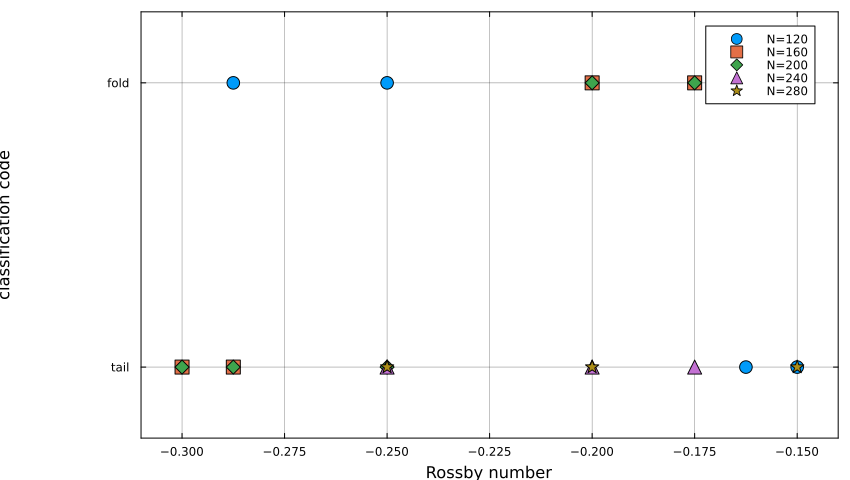
\includegraphics[width=0.88\textwidth]{../../work/results/presentation_evidence_audit_20260908/rossby_dense/summary/second_window_grid_sensitivity.png}
\caption{consistent模型较小$|\Ro|$区域的跨网格分类。fold标记随$N$移动并在固定$\Ro$处消失，因而属于长尾欠分辨造成的表观结构。空缺表示该网格未采样该点。}
\end{figure}

\begin{keyresult}
正确的研究结论不是“一致闭合消除了Boussinesq鞍结”，而是：
\begin{equation*}
 \boxed{\text{密度--加速度闭合重新组织了finite fold、thermal tail、smooth与passive区域。}}
\end{equation*}
\end{keyresult}

\section{从二维fold延拓到$\eps$链}

旧温度方程的二参数fold延拓曾提示有限核心fold臂朝$H_\infty=0$失局域边界
逼近，但该二维结果已被温度系数修正取代，不能作为corrected定量证据。当前证据
来自统一负$\Ro$切片和固定$\eps$增广fold链；新的连续二维fold图及跨$N$cusp
检验仍待重算。因此目前只说“未建立物理cusp”，不把表观转向判死为数值伪影。

为了把“fold 向热尾边界靠近”变成可计算的问题，需要用一个有物理意义的小参数
标记每一个 fold。远场泵吸量正好趋于零，因此定义
\begin{equation}\label{eq:epsdef}
 \boxed{\eps=-H_\infty>0}
\end{equation}
在每个固定$\eps$，未知量不是单独的$\Ro$或$T_w$，而是
$X=(U,v,\Ro,T_w)$。实际求解
\begin{equation}\label{eq:topology_augfold}
 \R(U;\Ro,T_w)=0,\quad J_Uv=0,\quad
 v^\mathsf{T}v=1,\quad H_\infty(U)+\eps=0.
\end{equation}
若$U$有$n$个离散未知量，那么$X$有$2n+2$个未知量，式
\eqref{eq:topology_augfold}也恰有$2n+2$个标量方程。第一组给稳态解，第二组把
解限制在fold，第三组去掉$v$的任意倍数，第四组选择fold曲线上的具体位置。

计算从$\Ro=-0.5$的已知fold开始，依次取
\begin{equation*}
 \eps=0.10,\ 0.05,\ 0.02,\ 0.01,\ 0.005,
\end{equation*}
即令$H_\infty=-\eps$。每一步把上一个
$(U,v,\Ro,T_w)$作为Newton初值，重新同时校正所有未知量，而不是在旧数据间插值。
由此得到
\begin{center}
\begin{tabular}{ccc}
\toprule
$\eps$ & $\Ro_f(\eps)$ & $T_{w,f}(\eps)$\\
\midrule
$0.100$ & $-0.504279302$ & $1.698160170$\\
$0.050$ & $-0.486196705$ & $1.678187170$\\
$0.020$ & $-0.476425364$ & $1.667840323$\\
$0.010$ & $-0.473351138$ & $1.664651476$\\
$0.005$ & $-0.472088411$ & $1.663350911$\\
\bottomrule
\end{tabular}
\end{center}
上表是$N=320$离散值，而非逐位收敛坐标。$\eps=0.02$的$N=280$--$320$
位置较一致；$\eps=0.01$仍有非单调网格漂移，$\eps=0.005$明显分辨率敏感。
后两点只用于展示趋势，误差随尾长增加而放大。

\begin{figure}[htbp]
\centering

\includegraphics[width=0.9\textwidth]{epsilon_fold_chain.png}
\caption{以物理量$\eps=-H_\infty$参数化的fold数据链。}
\end{figure}

\section{数值标度}

五点数据支持
\begin{equation}\label{eq:fit}
 \Ro_f=\Ro_t+A_R\eps+B_R\eps^2+\cdots,
 \qquad T_{w,f}=T_{w,t}+A_T\eps+B_T\eps^2+\cdots.
\end{equation}
校正后的数据仍显示近似线性接近，但由于小$\eps$点受长尾分辨率影响，本文只把
$p=q=1$作为工作标度，不宣称新的高精度二次拟合。外层边值问题给出的极限候选为
\begin{align}
\Ro_t&\simeq-0.470367416,\\
 T_{w,t}&\simeq1.661587420.
\end{align}
这是归一化leading outer BVP的数值解，并由独立的$g$坐标算法复核到约
$2\times10^{-10}$；它不是有限$\eps$数据拟合，也不是完整奇异问题的存在唯一性
证明。有限$\eps$数据支持以下工作标度：
\begin{equation}
 \Ro-\Ro_t=\order(\eps),\qquad T_w-T_{w,t}=\order(\eps).
\end{equation}

旧的scaling拟合图对应未校正方程，已经撤下；请直接用上表和outer极限检查
线性工作标度。

\begin{keyresult}[：为什么下一章不再继续堆数值点]
fold链回答了“有限$\eps$时fold在哪里”，却没有回答三个新问题：
\begin{enumerate}
  \item 为什么$\eps$越小越难解析，真正发散的空间尺度是什么？
  \item $\Ro_f,T_{w,f}$是否趋于有限端点，端点由哪组边界条件选择？
  \item finite fold 的Jacobian零模怎样在失局域极限中继续存在？
\end{enumerate}
第一个问题产生$Y=\eps\eta$；第二个问题产生inner相容和outer BVP；第三个问题
产生完整fold切向与伴随。后续方程只为解决这三个缺口而推导。
\end{keyresult}

\enlargethispage{5\baselineskip}
\begin{checkpoint}
\begin{enumerate}
  \item 用自己的话解释“closure reorganises topology”比“fold disappears”强在哪里。
  \item 为什么$\eps=-H_\infty$比人为弧长更适合后续渐近分析？
  \item 哪些数字是直接fold解，哪些数字是$\eps\to0$外推？
\end{enumerate}
\end{checkpoint}

%=====================================================================
\part{为渐近分析补齐数学基础}

\chapter{从Taylor展开到奇异摄动}\label{ch:math}

\begin{learninggoal}{会读$O(\eps)$、理解非均匀极限，并知道何时必须引入新坐标}
本章只讲本项目需要的数学，不追求一般渐近分析教材的完整性。
\end{learninggoal}

本章先不求任何具体系数，只建立一套“看到小参数后该问什么”的工作顺序：
先定义极限对象，再检查导数阶数是否丢失，最后用尺度平衡决定坐标。这样后面
出现 inner 和 outer 时，读者已经知道它们是由失效的单一展开强制产生的，而不是
作者任意切换的两种方法。

\section{$O(\eps^p)$究竟是什么意思}

写$f(\eps)=O(\eps^p)$，表示存在与小$\eps$无关的常数$C$，使得充分小$\eps$下
$|f(\eps)|\le C\eps^p$。若进一步
\begin{equation}
 \lim_{\eps\to0}\frac{f(\eps)}{\eps^p}=A\ne0,
\end{equation}
则写$f\sim A\eps^p$。数值图上“看起来近似直线”只是提示；指数、窗口、离散误差
和残差阶都需要检查。

\section{正则与奇异摄动}

若把$\eps=0$代入后，方程阶数、边界条件数量和解的空间尺度都不变，通常是正则
摄动。若最高导数前出现小参数，例如
\begin{equation}
 \eps^4 f''+A(f,g,T)=0,
\end{equation}
令$\eps=0$会丢掉微分阶数，原边界条件无法全部由极限方程满足，这就是奇异摄动。

\section{先记录远场线索，暂不建立outer}

已知fold链用$\eps=-H_\infty>0$参数化。远场令$S=T'$，校正后的温度方程给
\begin{equation}
 S'+\Pran\Ro H_\infty S=0,
 \qquad
 S(\eta)=C\exp[\Pran\Ro\eps\eta].
\end{equation}
所研究分支满足$\Ro<0$，所以
\begin{equation}\label{eq:tail_hint}
 k_T=\Pran(-\Ro)\eps,
 \qquad
 L_T=\frac{1}{\Pran(-\Ro)\eps}=O(\eps^{-1}).
\end{equation}
这只告诉我们：完整解含有一个越来越长的远场尺度，组合$\eps\eta$将在后面出现。
此处尚未确定outer中各场的幅值，也尚未给出outer入口条件。

下一步先回到物理壁面附近，在固定$\eta=O(1)$下分析inner。inner的一阶项若随
$\eta$增长，就会独立暴露局部展开的失效尺度；届时再把它与式
\eqref{eq:tail_hint}相互核对，建立outer。这样每一步只使用此前已经得到的结果。

\section{隐函数定理、奇异值与零模}

若方阵$J$可逆，局部解对参数光滑。若最小奇异值$\sigma_{\min}(J)$趋零，存在单位
向量$v$使$\|Jv\|$很小。SVD比直接看行列式稳健，因为行列式把所有奇异值相乘，
对尺度极敏感。仓库报告的是行缩放Jacobian的奇异值；它是固定离散下的可重复诊断，
不是有量纲物理量。

\begin{checkpoint}
\begin{enumerate}
  \item 举例说明“固定$\eta$极限”和“固定$Y$极限”得到不同答案。
  \item 为什么最高导数前的$\eps^4$比$\eps$本身更值得警惕？
  \item $\sigma_{\min}\ll1$和严格$Jv=0$之间还差哪些数值验证？
\end{enumerate}
\end{checkpoint}

%=====================================================================
\part{奇异fold--tail极限的逐步推导}

\chapter{退化inner core与解析相容曲线}\label{ch:inner}

\begin{learninggoal}{从固定$\eta$标度推出零阶核心与一阶参数方向}
本章要亲手推出$T_w=\Tcurve(\Ro)$以及$A_T/A_R=\Tcurve'(\Ro_t)$。
\end{learninggoal}

本章只固定 $\eta=O(1)$，所以先看壁面附近。推导严格按四步进行：
\begin{enumerate}
  \item 写出每个场的 inner 量级；
  \item 代入连续性和温度/方位方程，得到线性函数；
  \item 将径向方程的 $O(1)$ 项设为零，得到相容曲线；
  \item 再比较 $O(\eps)$ 的常数项，得到参数方向，但暂不求绝对切向大小。
\end{enumerate}
本章不使用尚未建立的outer入口条件。先由有限$\eps$剖面提出固定$\eta$下的候选
量级，再把它们代回原方程逐阶检验。末尾出现的线性增长将告诉我们局部展开在哪里
失效；下一章才根据这个失效尺度和远场热尾线索建立outer。

\section{inner展开}

有限$\eps$的fold剖面在若干固定$\eta$处显示：$G$和$T-T_{w,t}$随$\eps$
近似线性减小，$F,H$约按$\eps^2$减小；完整增广fold切向还提示两参数修正为
$O(\eps)$。这些是提出展开的数值线索，不是渐近证明。因此先写候选形式
\begin{subequations}\label{eq:innerexp}
\begin{align}
 G&=\eps G_1+\eps^2G_2+\cdots,\\
 T&=T_{w,t}+\eps\Theta_1+\eps^2\Theta_2+\cdots,\\
 F&=\eps^2F_2+\cdots,\\
 H&=\eps^2H_2+\cdots,\\
 \Ro&=\Ro_t+\eps r_1+\cdots,\\
 T_w&=T_{w,t}+\eps\tau_1+\cdots.
\end{align}
\end{subequations}
这里$r_1=A_R,\tau_1=A_T$。接下来检查这组幂次是否使各方程逐阶相容；若出现
无法平衡的项，就必须修改候选展开。它在inner方程中自洽仍不等于全域有效，远端
行为将决定是否还需要新坐标。

\begin{derivationbox}[：代入inner方程前的逐项阶数表]
inner坐标$\eta$本身不随$\eps$缩放，所以对$\eta$求导不改变$\eps$幂次。各项为
\begin{center}
\begin{tabular}{p{0.25\textwidth}p{0.22\textwidth}p{0.38\textwidth}}
\toprule
方程 & 最低微分项 & 最低非线性/输运项\\
\midrule
$H'+2F=0$ & $H'=O(\eps^2)$ & $F=O(\eps^2)$\\
温度 & $T''=O(\eps)$ & $HT'=O(\eps^3)$\\
方位 & $G''=O(\eps)$ & $F=O(\eps^2)$，$HG'=O(\eps^3)$\\
径向 & $F''=O(\eps^2)$ & 旋转代数项先有$O(1)$，再有$O(\eps)$\\
\bottomrule
\end{tabular}
\end{center}
因此温度和方位方程在最先出现的$O(\eps)$只剩二阶导数；径向方程则必须先令
$O(1)$代数项消失，再在$O(\eps)$得到参数与入口斜率相容条件。这个次序解释了
下面每一条方程从哪一阶取得。
\end{derivationbox}

\section{零阶退化核心}

连续性给$H_2'+2F_2=0$。温度和方位方程在$O(\eps)$分别给
\begin{equation}
 \Theta_1''=0,\qquad G_1''=0,
\end{equation}
所以利用壁面条件可写
\begin{equation}\label{eq:innerlinear}
 \Theta_1=\tau_1+B_T\eta,\qquad G_1=B_G\eta.
\end{equation}

\begin{derivationbox}[：径向代数项从$O(1)$展开到$O(\eps)$]
先只展开径向方程中可能为$O(1)$的部分
\begin{equation*}
 \frac{\omega^2-\chi(T)(s+\Ro G)^2}{\Ro}.
\end{equation*}
沿fold链有
\begin{align*}
 \Ro&=\Ro_t+\eps r_1+O(\eps^2),\\
 s&=s_t+\eps s_t'r_1+O(\eps^2),\\
 \omega&=\omega_t+\eps\omega_t'r_1+O(\eps^2),\\
 \chi(T)&=\chi_t-\eps\gamma\Theta_1+O(\eps^2),\\
 s+\Ro G&=s_t+\eps(s_t'r_1+\Ro_tG_1)+O(\eps^2).
\end{align*}
分别平方并相乘：
\begin{align*}
 \omega^2
 &=\omega_t^2+2\eps\omega_t\omega_t'r_1+O(\eps^2),\\
 \chi(s+\Ro G)^2
 &=\chi_ts_t^2+\eps\left[
 2\chi_ts_t(s_t'r_1+\Ro_tG_1)-\gamma s_t^2\Theta_1
 \right]+O(\eps^2).
\end{align*}
因为分子的$O(1)$项随后会被令为零，$1/\Ro$自身的$O(\eps)$修正不会进入下一阶。
径向黏性和径向惯性从$O(\eps^2)$才开始，也不进入以下两阶。
\end{derivationbox}

于是径向方程的$O(1)$项要求
\begin{equation}\label{eq:corecompat}
 \boxed{\chi(T_{w,t})s_t^2=\omega_t^2.}
\end{equation}
因此
\begin{equation}
 F_0=G_0=H_0=0,\qquad T_0=T_{w,t}
\end{equation}
是leading inner问题的精确候选解：壁面附近的$O(1)$流动核心塌缩，温度和方位
速度的$O(1)$变化被推到慢外层。

由式\eqref{eq:corecompat}得到解析相容曲线
\begin{equation}\label{eq:tcurve}
 \boxed{
 \Tcurve(r)=1+\frac1\gamma\left[1-\left(\frac{\omega(r)}{s(r)}\right)^2\right].}
\end{equation}
校正后的 outer 极限候选为
$\Ro_t\simeq-0.470367416$、$T_{w,t}\simeq1.661587420$。相容曲线仍提供
必要的参数关系，但当前数据不足以把它当作独立的高精度唯一性验证。

\begin{evidencebox}[：强数值一致性，但不是唯一性定理]
固定$\eta=1,2,5$处，最后两个$\eps$点显示$F,H$约按$\eps^2$衰减，$G$和
$T_w-T$约按$\eps$衰减；核心缺陷
$\chi(T_w)s^2-\omega^2$沿fold链系统趋零。这支持分支选择退化零核心，但有限五点
不能排除所有非正则overlap或证明极限解唯一。
\end{evidencebox}

\section{一阶径向相容条件}

记
\begin{equation}
 s_t'=-\frac12-\Ro_t,\qquad \omega_t'=\frac12-\Ro_t,
\end{equation}
以及
\begin{equation}
 D_t'=2\omega_t\omega_t'-2\chi_t s_t s_t'.
\end{equation}
把上一个推导框中$O(\eps)$系数收集起来，径向代数平衡为
\begin{equation}\label{eq:innercompat1}
 \gamma s_t^2\Theta_1-2\chi_t s_t\Ro_tG_1+D_t'r_1=0.
\end{equation}
代入式\eqref{eq:innerlinear}并分别比较常数项和$\eta$项：
\begin{subequations}
\begin{align}
 \gamma s_t^2\tau_1+D_t'r_1&=0,\\
 \gamma s_t^2B_T-2\chi_t s_t\Ro_tB_G&=0.
\end{align}
\end{subequations}
第一式给
\begin{equation}\label{eq:slopeinner}
 \boxed{\frac{\tau_1}{r_1}=-\frac{D_t'}{\gamma s_t^2}=\Tcurve'(\Ro_t).}
\end{equation}
因此inner分析决定的是参数平面中的方向，不决定$r_1$的绝对大小。

\section{inner怎样暴露自己的失效尺度}

到这里我们只求了固定$\eta=O(1)$的局部解。式\eqref{eq:innerlinear}给
\begin{equation}
 G\sim\eps B_G\eta,
 \qquad
 T-T_{w,t}\sim\eps\tau_1+\eps B_T\eta.
\end{equation}
若$B_G,B_T$为有限非零常数，则在$\eps\eta\ll1$时，这些空间变化确实是小修正；
当
\begin{equation}\label{eq:inner_breakdown}
 \eps\eta=O(1),\qquad\text{即}\qquad \eta=O(\eps^{-1}),
\end{equation}
它们成长为$O(1)$，固定$\eta$展开失去阶次分离。inner因此不能独自满足
$G(\infty)=1$和$T(\infty)=1$；未知系数$B_G,B_T$也不能由局部壁面问题决定。

这个失效尺度与式\eqref{eq:tail_hint}由远场指数得到的热尾长度完全一致。两条相互
独立的线索共同要求下一章引入$Y=\eps\eta$。到目前为止尚未施加任何outer入口
条件，也尚未进行匹配。

\begin{checkpoint}
\begin{enumerate}
  \item 从式\eqref{eq:tcurve}直接求导，验证它等于式\eqref{eq:slopeinner}。
  \item 为什么$G_1\propto\eta$不是“inner解在无穷远发散”的错误？
  \item 相容曲线为什么不能单独选出$\Ro_t$？
  \item 哪两个独立计算同时给出$\eta=O(\eps^{-1})$？
\end{enumerate}
\end{checkpoint}

%=====================================================================
\chapter{thermo--rotational slow tail与outer DAE}\label{ch:outer}

\begin{learninggoal}{逐项推出$Y=\eps\eta$上的outer方程，并理解极限点如何被选择}
本章是整项研究最核心的多尺度结构。
\end{learninggoal}

上一章已经由inner线性增长得到失效尺度$\eta=O(\eps^{-1})$；第七章的远场热模
给出同一尺度。本章依次完成“定义$Y$--确定各场幅值--代入方程--消去代数约束”。
等inner和outer两侧表达式都已建立以后，才定义overlap、完成匹配并施加outer边界
条件。这个顺序避免提前借用尚未推导的入口值。

\section{先从温度尾长开始}

远处取$H\to-\eps$，温度方程线性化为
\begin{equation}
 T''-\Pran\Ro\eps T'=0,
\end{equation}
所以
\begin{equation}
 T-1\sim C\exp(\Pran\Ro\eps\eta),
 \qquad \boxed{L_T\sim\frac1{\Pran(-\Ro)\eps}}\quad(\Ro<0).
\end{equation}
这迫使我们取$Y=\eps\eta$。但若在整个outer区都令$F=0,G=1,H=-\eps$，而
$T-1=O(1)$，一致模型径向残差一般不为零。因此它不只是“温度拖出长尾”，而是
温度和方位速度共同调整的\textbf{热--旋转慢尾}。

\section{distinguished outer scaling}

式\eqref{eq:inner_breakdown}要求在新区域保持$Y=\eps\eta=O(1)$。在整条慢尾上，
$G$必须从近壁核心值趋向远场值$1$，$T$也必须从$T_{w,t}$趋向$1$；两者的总跳跃
均为$O(1)$，故取$G=g(Y)=O(1)$、$T=\theta(Y)=O(1)$。定义
$H_\infty=-\eps$给出$H=\eps h(Y)$且$h(\infty)=-1$。最后由连续性
$H'+2F=0$得到$H'=O(\eps^2)$，所以$F=O(\eps^2)$。因此取
取
\begin{equation}\label{eq:outerscaling}
 Y=\eps\eta,\qquad
 F=\eps^2 f(Y),\quad H=\eps h(Y),\quad G=g(Y),\quad T=\theta(Y).
\end{equation}

\begin{derivationbox}[：先做导数账本，再代入方程]
在本框内，下标 $Y$ 表示对 $Y$ 求导。由链式法则逐项得到
\begin{center}
\begin{tabular}{cccc}
\toprule
场 & 原量级 & 一阶 $\eta$ 导数 & 二阶 $\eta$ 导数\\
\midrule
$F$ & $\eps^2f$ & $\eps^3f_Y$ & $\eps^4f_{YY}$\\
$H$ & $\eps h$ & $\eps^2h_Y$ & $\eps^3h_{YY}$\\
$G$ & $g$ & $\eps g_Y$ & $\eps^2g_{YY}$\\
$T$ & $\theta$ & $\eps\theta_Y$ & $\eps^2\theta_{YY}$\\
\bottomrule
\end{tabular}
\end{center}
然后逐个方程代入，而不是凭直觉删项：
\begin{align*}
 H'+2F&=\eps^2(h_Y+2f),\\
 T''+\Pran\Ro H T'&=\eps^2(\theta_{YY}+\Pran\Ro h\theta_Y),\\
 G''+\chi\{\Ro(2FG+HG')+\Co F\}
 &=\eps^2\!\left[g_{YY}+\chi\{\Ro(2fg+hg_Y)+\Co f\}\right].
\end{align*}
三个式子除以共同因子 $\eps^2$ 后仍保留微分阶数。径向方程不同：
$F''=\eps^4f_{YY}$，而离心/压力代数项是 $O(1)$；因此 $\eps\to0$ 时径向
微分项先消失，留下慢流形约束。这正是 DAE 出现的原因。
\end{derivationbox}

将前三个式子除以$\eps^2$，并在leading问题中令参数趋于$\Ro_t$，连续性、
温度和方位动量分别给
\begin{subequations}\label{eq:outerfull}
\begin{align}
 h'+2f&=0,\\
 \theta''+\Pran\Ro_t h\theta'&=0,\\
 g''+\chi(\theta)\left[\Ro_t(2fg+hg')+2s_tf\right]&=0.
\end{align}
\end{subequations}
若保留fold链上的参数依赖$\Ro_\eps=\Ro(\eps)$，并记
$s_\eps=s(\Ro_\eps),\omega_\eps=\omega(\Ro_\eps)$，径向方程精确变成
\begin{equation}\label{eq:outerradialeps}
 \eps^4\left[f''+\chi\Ro_\eps(f^2+hf')\right]
 +\frac{\omega_\eps^2-\chi(\theta)(s_\eps+\Ro_\eps g)^2}{\Ro_\eps}=0.
\end{equation}
这里没有把有限-$\eps$参数提前冻结：$\Ro_\eps,s_\eps,\omega_\eps$仍沿 fold 链
变化。式中第一组括号乘 $\eps^4$，第二组一般是 $O(1)$。若解族在极限中保持有界，
则两步极限为
\begin{align*}
 \Ro_\eps&\longrightarrow\Ro_t,\qquad
 s_\eps\longrightarrow s_t,\qquad \omega_\eps\longrightarrow\omega_t,\\
 \eps^4\left[f''+\chi\Ro_\eps(f^2+hf')\right]&\longrightarrow0.
\end{align*}
因此剩余的 $O(1)$ 代数项必须单独为零，留下
\begin{equation}\label{eq:slowmanifold}
 \boxed{\chi(\theta)(s_t+\Ro_tg)^2=\omega_t^2.}
\end{equation}

\section{为什么这是DAE和slow manifold}

式\eqref{eq:outerfull}含微分方程，式\eqref{eq:slowmanifold}是代数方程，所以极限
系统是differential--algebraic equation（DAE）。它把$g$和$\theta$限制在
\begin{equation}\label{eq:thetaofg}
 \theta(g;r)=1+\frac1\gamma\left[1-\frac{\omega(r)^2}{(s(r)+rg)^2}\right]
\end{equation}
上。这里“slow manifold”只表示代数约束曲线；尚未证明动力系统意义下的法向
双曲性或吸引性。

\section{化成可求解的三个一阶ODE}

令$q=s+rg$、$p=g'$。下面把消元过程完整写出。

\begin{derivationbox}[：从 DAE 到三个一阶 ODE]
第一步，由慢流形先把温度写成 $g$ 的函数：
\begin{equation*}
 \theta(g)=1+\frac1\gamma\left(1-\frac{\omega^2}{q^2}\right),\qquad
 \chi=\frac{\omega^2}{q^2},\qquad
 \theta_g=\frac{2r\omega^2}{\gamma q^3}.
\end{equation*}
记 $A(g)=\theta_g$，则 $A_g=-3rA/q$，并且
\begin{equation*}
 \theta_Y=Ap,\qquad \theta_{YY}=A p'-\frac{3rA}{q}p^2.
\end{equation*}
代入温度方程 $\theta_{YY}+\Pran r h\theta_Y=0$，除以非零的 $A$，得到
\begin{equation*}
 p'=\frac{3rp^2}{q}-\Pran r hp.
\end{equation*}
第二步，连续性给 $f=-h'/2$。把它代入方位方程：
\begin{align*}
 0&=p'+\chi\{r(2fg+hp)+2sf\}\\
  &=p'+\chi\{rhp+2f(s+rg)\}\\
  &=p'+\chi(rhp-qh').
\end{align*}
解出 $h'$ 即得第三个方程。整个约化没有再引入经验闭合。
\end{derivationbox}

于是可求解系统为
\begin{subequations}\label{eq:outerreduced}
\begin{align}
 g'&=p,\\
 p'&=\frac{3rp^2}{q}-\Pran r hp,\\
 h'&=\frac{p'+\chi rhp}{\chi q},
 \qquad \chi=\frac{\omega^2}{q^2}.
\end{align}
\end{subequations}

\section{两侧都已得到后再做匹配}\label{sec:matching}

对每一个固定$\eps>0$，物理上只有同一个解$U(\eta;\eps)$。inner是在固定
$\eta=O(1)$下观察它，outer是在固定$Y=\eps\eta=O(1)$下观察它。要让两种表示
描述同一个解，需要一段同时满足
\begin{equation}\label{eq:overlap}
 1\ll\eta\ll\eps^{-1}
\end{equation}
的重叠区。严格地，任选$0<\alpha<1$并令$\eta=\eps^{-\alpha}$，则
$\eta\to\infty$而$Y=\eps^{1-\alpha}\to0$。所以匹配比较的是inner的远端共同
部分与outer的入口共同部分。

假设leading outer解在$Y=0$正则，写
\begin{subequations}\label{eq:outerentrance}
\begin{align}
 g(Y)&=g_0+p_0Y+O(Y^2),\\
 \theta(Y)&=\theta_0+\theta_1Y+O(Y^2),\\
 h(Y)&=h_0+h_1Y+O(Y^2),\\
 f(Y)&=f_0+O(Y).
\end{align}
\end{subequations}
现在逐项与第八章已经求得的inner展开比较：

\begin{itemize}
  \item $G^{\mathrm{in}}\sim\eps B_G\eta=B_GY$，故
  $g_0=0$且$p_0=B_G$；
  \item $T^{\mathrm{in}}\sim T_{w,t}+\eps\tau_1+B_TY$，故leading阶有
  $\theta_0=T_{w,t}$、$\theta_1=B_T$。其中$\eps\tau_1$属于下一阶outer入口
  常数，不能塞进leading的$\theta_0$；
  \item $H^{\mathrm{in}}=\eps^2H_2$。若$H_2$在重叠区至多线性增长，则与
  $H^{\mathrm{out}}=\eps(h_0+h_1Y+\cdots)$比较给
  $h_0=0$和$H_2\sim h_1\eta$；
  \item $F^{\mathrm{in}}=\eps^2F_2(\eta)$，而
  $F^{\mathrm{out}}=\eps^2[f_0+O(Y)]$，所以正确的匹配是
  \begin{equation}\label{eq:Fmatching}
    F_2(\eta)\longrightarrow f_0
    \qquad(\eta\to\infty\ \text{的匹配意义下}).
  \end{equation}
  $f_0$只是inner远端的共同部分，不是整个函数$F_2(\eta)$；物理壁面仍满足
  $F_2(0)=0$。
\end{itemize}

连续性在入口还给$h_1+2f_0=0$。特别要注意，outer的$Y=0$是
$\eps\to0$时从慢尾一侧接近inner远端的极限，不能把它等同于固定$\eps$时的
物理壁面$\eta=0$。

因此leading outer问题的入口值为
\begin{equation}\label{eq:outerentrancebc}
 g(0)=0,\qquad \theta(0)=T_{w,t},\qquad h(0)=0,
\end{equation}
而$f(0)=f_0$一般不为零。这里关于$H_2$增长的正则性是假设；现有有限$\eps$
剖面支持它，但尚无严格一致误差界。

\section{远场条件选择outer端点}

采用的匹配/归一化条件是
\begin{equation}\label{eq:outerbc}
 g(0)=0,\quad h(0)=0,\qquad
 g(\infty)=1,\quad h(\infty)=-1.
\end{equation}
其中$h(\infty)=-1$由定义$H_\infty=-\eps$严格给出；两个入口值则由上一节的
共同部分匹配得到。代数约束式\eqref{eq:thetaofg}自动给
$\theta(0)=T_{w,t}$，所以约化的一阶系统不必再把它列成独立边界条件。

未知初始斜率$p(0)$和参数$r$由两个远场条件共同选出：
\begin{align}
 \boxed{\Ro_t\simeq-0.470367416},\qquad
 \boxed{T_{w,t}\simeq1.661587420},\qquad
 \boxed{g'(0)\simeq0.654193539}.
\end{align}
把$g$本身改作独立变量的第二种积分算法得到相同三数，与上述$Y$坐标shooting
结果相差约$2\times10^{-10}$。这是约化问题的独立数值核验，不是完整fold链的
$\eps\to0$误差界。

还可以直接检查完整finite-$\eps$基本流是否逼近该outer剖面。对$N=320$数据在
$0\le Y\le10$计算relative-$L^2$误差，得到
\begin{center}
\begin{tabular}{cccc}
\toprule
$\eps$ & $G$ & $T$ & $H/\eps$\\
\midrule
$0.020$ & $0.407\%$ & $0.148\%$ & $0.815\%$\\
$0.010$ & $0.175\%$ & $0.093\%$ & $0.406\%$\\
\bottomrule
\end{tabular}
\end{center}
误差随$\eps$减小而系统下降，为leading outer基本流提供了比“端点坐标接近”更强的
剖面证据。这里没有列$F$，因为leading outer中的$F=\eps^2f$及其inner入口过渡
需要单独处理；本表也不含fold零模，后者由下一章的增广系统检查。

\section{为什么outer BVP正则并不矛盾}

对shooting残差$(g(Y_{\max})-1,h(Y_{\max})+1)$关于$(p(0),r)$求Jacobian，得到
\begin{equation}
 \sigma_{\min}=0.9817203,\quad \sigma_{\max}=5.4207957,\quad
 \kappa=5.5217312,\quad \det J=5.3217051.
\end{equation}
这些是corrected方程在$Y_{\max}=60$的$2\times2$ shooting Jacobian诊断，不是
full BVP的谱或稳定性特征值。它们说明该归一化leading outer根局部孤立。它的任务是选择极限状态，不是保留
有限$\eps$固定$T_w$基本流Jacobian的普通零模。

\begin{warningbox}
“full finite-$\eps$ system有fold”与“reduced leading outer BVP正则”不冲突。
两者不是同一个算子，且full零模各分量在极限中需要不同重缩放。先降阶再线性化与
先线性化再作奇异极限这两种操作不交换。
\end{warningbox}

\begin{checkpoint}
\begin{enumerate}
  \item 从式\eqref{eq:thetaofg}和能量方程独立推出$p'$方程。
  \item 为什么径向黏性项前恰好是$\eps^4$？
  \item $h(\infty)=-1$如何固定了$\eps$的绝对尺度？
\end{enumerate}
\end{checkpoint}

%=====================================================================
\chapter{完整增广fold切向、伴随与两级选择}\label{ch:tangent}

\begin{learninggoal}{理解极限位置、离开方向和绝对速度分别由谁决定}
这是把数值分岔与渐近理论闭合起来的一章。
\end{learninggoal}

本章解决一个容易被混淆的问题：极限点、参数平面方向和有限-$\eps$离开速度不是
同一个量。先用增广 fold 方程求完整切向，再用左零模验证可解性，最后与 outer
相容曲线的斜率比较。没有这三个层次，不能把一张有限-$\eps$表格外推成
$A_R,A_T$ 的极限定理。

还必须明确：第八、九章只把满足基本流方程的解带到 $\eps\to0$，其中没有
$J_Uv=0$，所以它们单独描述的是长尾极限，不能单独证明该长尾位于fold链上。
真正加入fold约束的是本章式\eqref{eq:augfold}。因此本文采用的联系证据是：
finite-$\eps$增广fold解的位置趋向outer端点、参数切向趋向inner相容曲线的切线，
并检查零模在慢坐标上的分量结构。这个联合证据支持fold--tail连接，但尚不是带统一
误差界的匹配存在定理。

\section{完整增广系统}

有限$\eps$的fold由
\begin{equation}\label{eq:augfold}
 \mathcal F_{\mathrm{aug}}(U,T_w,v,\Ro;\eps)=
 \begin{pmatrix}
  \R(U,\Ro,T_w)\\
  J_Uv\\
  v^\mathsf{T}v-1\\
  H_\infty(U)+\eps
 \end{pmatrix}=0
\end{equation}
定义。四行依次表示：基本流成立、固定$T_w$ Jacobian有右零模、零模归一化、
以及用物理量$\eps=-H_\infty$参数化奇异点链。它们给出fold候选；称为简单fold
还要检查核维数、$\langle w,\R_{T_w}\rangle\ne0$、
$\langle w,\R_{UU}[v,v]\rangle\ne0$及完整增广Jacobian可逆。

\section{对$\eps$求导}

令$Z=(U,T_w,v,\Ro)$，则
\begin{equation}
 D_Z\mathcal F_{\mathrm{aug}}\,Z_\eps=-(0,\ldots,0,1)^\mathsf{T}.
\end{equation}
其中基本流切向方程为
\begin{equation}\label{eq:basetangent}
 J_UU_\eps+\R_\Ro\Ro_\eps+\R_{T_w}T_{w,\eps}=0,
\end{equation}
零模方程的导数还包含方向Hessian
\begin{equation}
 J_Uv_\eps+\R_{UU}[U_\eps,v]
 +\Ro_\eps\R_{U\Ro}v+T_{w,\eps}\R_{UT_w}v=0.
\end{equation}
归一化与$H_\infty$约束给
\begin{equation}
 v^\mathsf{T}v_\eps=0,\qquad (H_\infty)_\eps=-1.
\end{equation}
若这些导数存在且$\eps$是有效局部坐标，则定义
\begin{equation}
 A_R=\lim_{\eps\to0}\Ro_\eps,\qquad
 A_T=\lim_{\eps\to0}T_{w,\eps}.
\end{equation}

\section{左零模与伴随可解性}

设
\begin{equation}
 J_U^\mathsf{T}w=0.
\end{equation}
用$w^\mathsf{T}$左乘式\eqref{eq:basetangent}，第一项消失，得到
\begin{equation}\label{eq:adjointslope}
 \boxed{
 \frac{T_{w,\eps}}{\Ro_\eps}
 =-\frac{\langle w,\R_\Ro\rangle}{\langle w,\R_{T_w}\rangle}.}
\end{equation}
数值中两边在所有计算点一致到约$10^{-11}$，并趋向
\begin{equation}
 \Tcurve'(\Ro_t)\simeq-1.021771561.
\end{equation}
这里的$10^{-11}$量级检查的是同一离散系统中的直接切向与伴随恒等式，不能当作
到$\eps=0$渐近斜率的误差。$N=320$时，$\eps=0.02,0.015,0.01$的斜率距
式\eqref{eq:slopeinner}的极限值仍约$2.03\%,1.52\%,1.01\%$。其系统趋近支持
inner相容、解析曲线切线与full-system伴随投影具有同一极限方向。

\section{两级选择机制}

\begin{keyresult}
\begin{enumerate}
 \item 归一化leading outer BVP由整组入口/远场条件选择极限位置
 $(\Ro_t,T_{w,t})$，其中$h(\infty)=-1$固定尺度；
 \item 相容曲线/伴随关系选择参数平面方向$A_T/A_R$；
 \item 完整增广fold切向连同$(H_\infty)_\eps=-1$给出有限$\eps$绝对速度；
 若其极限存在并收敛，才定义$(A_R,A_T)$。
\end{enumerate}
这就是“两级选择”：先选终点，再由完整fold系统选离开终点的速度。
\end{keyresult}

\section{数值幅值与可信窗口}

$N=280$和$N=320$时（corrected energy）
\begin{center}
\begin{tabular}{ccccc}
\toprule
$\eps$ & $\Ro_\eps^{(280)}$ & $\Ro_\eps^{(320)}$ &
$T_{w,\eps}^{(280)}$ & $T_{w,\eps}^{(320)}$\\
\midrule
$0.020$ & $-0.311684464$ & $-0.312165536$ & $0.324935820$ & $0.325437335$\\
$0.015$ & $-0.307140323$ & $-0.306716465$ & $0.318581648$ & $0.318143353$\\
$0.010$ & $-0.314631752$ & $-0.310331167$ & $0.324725723$ & $0.320275829$\\
\bottomrule
\end{tabular}
\end{center}
$\eps=0.02,0.015$的两张最高网格差约$0.14\%$--$0.15\%$，支持这两个有限
$\eps$点的空间一致性；$\eps=0.01$差异约$1.37\%$，绝对切向尚未收敛。
各$N$结果也不是单调序列，因此当前不对$\eps\to0$外推，不报告新的$A_R,A_T$
极限值。旧温度方程的$(-0.4187145,0.5087672)$已经废止。

\section{fold零模的outer分量尺度：哪些已经验证，哪些尚未}

把右零模按$\max|v_G|=1$归一化，得到
\begin{equation}\label{eq:modescaling}
 v_G,v_T=O(1),\qquad v_H=O(\eps),\qquad v_F=O(\eps^2).
\end{equation}
在$Y=\eps\eta$上比较
\begin{equation}
 v_G,\quad v_T,\quad v_H/\eps,\quad v_F/\eps^2,
\end{equation}
校正后的$N=320$数据为
\begin{center}
\begin{tabular}{ccc}
\toprule
$\eps$ & $\max|v_H|/\max|v_G|$ & $\max|v_F|/\max|v_G|$\\
\midrule
$0.020$ & $0.07183$ & $1.748\times10^{-3}$\\
$0.015$ & $0.05381$ & $1.001\times10^{-3}$\\
$0.010$ & $0.03584$ & $4.535\times10^{-4}$\\
\bottomrule
\end{tabular}
\end{center}
这支持式\eqref{eq:modescaling}的分量幅值阶数；它没有证明
不同$\eps$的完整profile在某个函数范数下收敛。进一步以$\eps=0.01$为参考，
在$0\le Y\le10$上直接计算relative-$L^2$差，得到
\begin{center}
\begin{tabular}{ccccc}
\toprule
$\eps$ & $v_G$ & $v_T$ & $v_H/\eps$ & $v_F/\eps^2$\\
\midrule
$0.020$ & $0.987\%$ & $0.716\%$ & $0.313\%$ & $12.03\%$\\
$0.015$ & $0.527\%$ & $0.376\%$ & $0.159\%$ & $6.75\%$\\
\bottomrule
\end{tabular}
\end{center}
所以$G,T,H$分量已经显示清楚的emerging collapse，而$F/\eps^2$仍有明显差异；
现阶段不能声称四分量本征函数已经统一收敛。较弱的、由数据支持的表述是：full零模
并未在极限中简单消失，其主导慢尾分量具有与outer尺度相容的重标度；径向分量的
函数极限仍需更高分辨率或tail-adapted线性化BVP确认。这足以说明“正则leading
outer BVP”与“奇异finite-$\eps$ full Jacobian”在逻辑上不矛盾，但不把两者的
严格谱极限当作已完成定理。

\enlargethispage{4\baselineskip}
\begin{checkpoint}
\begin{enumerate}
  \item 从式\eqref{eq:basetangent}推出式\eqref{eq:adjointslope}。
  \item 为什么伴随只给参数方向，$H_\infty+\eps=0$还要给绝对速度？
  \item 用“极限操作不交换”解释式\eqref{eq:modescaling}的意义。
\end{enumerate}
\end{checkpoint}

%=====================================================================
\chapter{表观cusp为何必须先做分辨率检验}

\begin{learninggoal}{学会把数值伪结构与物理分岔区分开}
本章把热尾尺度和无限映射节点尺度连接起来。
\end{learninggoal}

热尾要求解析$L_T=O(\eps^{-1})$，而映射最后有限节点只到
$\eta_{N-1}=O(N^2)$。因此临界解析条件自然是
\begin{equation}
 \eps\eta_{N-1}=O(1)
 \quad\Longrightarrow\quad
 \boxed{\eps_{\min}=O(N^{-2}).}
\end{equation}
旧实测表和cusp-like图来自未校正温度方程，不能继续作为定量证据。上面的
$N^{-2}$关系仍是映射节点可达尺度的解析估计；它是否准确描述corrected fold链，
需要新的跨$N$数据检验。

\begin{evidencebox}
现有corrected证据支持“固定$\eps$ fold链接近远场失局域层”，尚未在有限参数处
建立物理cusp。corrected链没有新的cusp跨$N$拟合，所以也不能用本章的节点尺度
估计严格排除所有cusp。严格的$\eps=0$连接定理和统一误差估计仍未完成。
\end{evidencebox}

%=====================================================================
\part{把理论与Julia仓库连起来}

\chapter{代码导航与方程--实现对照}\label{ch:code}

\begin{learninggoal}{知道每个科学结论由哪段Julia代码和哪份结果支撑}
本章按“共享模块--执行脚本--输出--报告”四层组织。
\end{learninggoal}

\section{三个共享模块}

\begin{longtable}{p{0.27\textwidth}p{0.64\textwidth}}
\toprule
文件 & 作用\\
\midrule
\endfirsthead
\toprule
文件 & 作用\\
\midrule
\endhead
\path{work/src/BEKIsothermal.jl} & 构造Chebyshev--Pier映射、等温BEK残差、解析Jacobian和阻尼Newton。\\
\path{work/src/BEKThermal.jl} & 传统盘系固定离心热闭合；固定$T_w$、固定$H_\infty$及伪弧长求解；$\Ro=0$显式拒绝。\\
\path{work/src/BEKConsistent.jl} & 一致热残差、解析Jacobian、$\Ro$导数、方向Hessian、fold校正、二参数fold延拓与$H_\infty$参数化切向。\\
\bottomrule
\end{longtable}

\section{关键函数在数学上做什么}

\begin{longtable}{p{0.34\textwidth}p{0.56\textwidth}}
\toprule
Julia函数 & 数学对象\\
\midrule
\endfirsthead
\toprule
Julia函数 & 数学对象\\
\midrule
\endhead
\path{_residual_jacobian} & 同时返回$\R(U)$和$J_U$；边界行在这里替换。\\
\path{solve_consistent_fixed_tw} & 给定$(\Ro,T_w)$解$\R(U)=0$。\\
\path{solve_consistent_fixed_h} & 给定$(\Ro,H_\infty)$，把$T_w$作为未知量。\\
\path{solve_consistent_pseudoarclength} & 增加弧长条件跨越固定$T_w$ fold。\\
\path{solve_consistent_fold} & 解$\R=0,J_Uv=0,v^Tv=1$。\\
\path{solve_consistent_fold_at_h} & 再加$H_\infty$约束并释放$\Ro$。\\
\path{continue_consistent_fold} & 在完整状态、零模和参数空间中做fold伪弧长。\\
\path{fold_hinf_tangent} & 解式\eqref{eq:augfold}对$\eps$的隐式导数。\\
\bottomrule
\end{longtable}

\section{建议的复现顺序}

从仓库根目录使用Julia 1.10或更高版本（当前环境为Julia 1.12.7）：
\begin{lstlisting}[language=bash]
julia work/scripts/gate1_bek_isothermal.jl
julia work/scripts/vonkarman_consistent_baseflow.jl
julia work/scripts/compare_traditional_consistent_topology.jl
julia work/scripts/consistent_epsilon_fold_chain.jl --degree=320
julia work/scripts/solve_outer_limit_and_jacobian.jl
julia work/scripts/audit_learning_manual_20260907.jl
julia work/scripts/corrected_manual_tangent_convergence_20260907.jl --degree=320
julia work/scripts/summarize_corrected_manual_tangent_20260907.jl
\end{lstlisting}
这些脚本运行成本差异很大。学习时先阅读对应\texttt{docs/*.md}和CSV，确认理解
输入输出，再决定是否重跑高$N$ fold校正。跨网格切向需要对$N=200,240,280,320$
分别运行倒数第二个脚本。不要向\texttt{baselines/}写新结果。旧的scaling、inner和
mode-collapse脚本仍读取未校正目录，不能直接用于当前定量结论。

\section{科学结论与证据文件}

\begin{longtable}{p{0.30\textwidth}p{0.30\textwidth}p{0.31\textwidth}}
\toprule
问题 & 主要文档 & 主要结果目录\\
\midrule
\endfirsthead
\toprule
问题 & 主要文档 & 主要结果目录\\
\midrule
\endhead
等温BEK与传统von K\'arm\'an回归 & \path{GATE1_ISOTHERMAL_BEK.md} & \path{gate1_isothermal/}\\
传统全家族可解性 & \path{FULL_BEK_TRADITIONAL_RESULTS.md} & \path{full_bek_traditional_availability/}\\
一致$\Ro$加密与跨网格拓扑 & \path{PRESENTATION_EVIDENCE_AUDIT_2026-09-08.md} & \path{presentation_evidence_audit_20260908/rossby_dense/}\\
两模型统一拓扑 & \path{PRESENTATION_EVIDENCE_AUDIT_2026-09-08.md} & \path{presentation_evidence_audit_20260908/rossby_dense/}\\
corrected方程审计 & \path{LEARNING_MANUAL_AUDIT_2026-09-07.md} & \path{learning_manual_audit_20260907/}\\
$\eps$ fold数据链 & \path{CORRECTED_ENERGY_RECOMPUTATION_2026-09-06.md} & \path{corrected_energy_epsilon_fold_chain/}\\
outer极限选择 & \path{CORRECTED_ENERGY_RECOMPUTATION_2026-09-06.md} & \path{corrected_energy_outer_limit/}\\
完整fold切向与分量幅值 & \path{CORRECTED_MANUAL_SUPPLEMENT_2026-09-07.md} & \path{corrected_manual_tangent_convergence_20260907/}\\
\bottomrule
\end{longtable}

\begin{warningbox}
仓库报告是证据边界的权威来源。若本手册中的数字与未来新增日志冲突，应保留旧结果，
在\texttt{docs/RESEARCH\_PROGRESS\_LOG.md}追加新条目并明确“supersede”，而不是
静默改写研究历史。
\end{warningbox}

%=====================================================================
\chapter{一条适合自学的四周路线}

\section{第一周：只做基本流与数值方法}

\begin{enumerate}
 \item 手推等温方程在$\Ro=-1,0,1$的形式；
 \item 读\texttt{BEKIsothermal.jl}中的映射和边界行替换；
 \item 画一张纸面流程图：参数$\to$算子$\to$Newton$\to$剖面$\to H_\infty$；
 \item 理解固定$T_w$、固定$H_\infty$和伪弧长三种求解方式的未知量差异。
\end{enumerate}

\section{第二周：重建两模型拓扑}

\begin{enumerate}
 \item 从有量纲量比值重新推出$\Lambda_D=\gamma\Co^2/(4\Ro)$；
 \item 比较式\eqref{eq:traditional}与\eqref{eq:consistent}在$T=1$和$T\ne1$的差异；
  \item 不看表格，自己根据corrected CSV为加密负$\Ro$切片标注smooth/fold/tail，
  并找出随$N$漂移的表观fold；
 \item 写一页说明：为什么“数学可解到$T_w=2$”不是“物理有效到$T_w=2$”。
\end{enumerate}

\section{第三周：只学inner和outer}

\begin{enumerate}
 \item 熟练做$\dd/\dd\eta=\eps\dd/\dd Y$的阶数换算；
 \item 从零推出式\eqref{eq:corecompat}、\eqref{eq:tcurve}和\eqref{eq:slopeinner}；
 \item 逐项推出式\eqref{eq:outerradialeps}中的$\eps^4$；
 \item 从slow manifold消去$\theta$，推出式\eqref{eq:outerreduced}；
 \item 用两句话区分overlap极限和真实远场。
\end{enumerate}

\section{第四周：fold切向、伴随与证据表达}

\begin{enumerate}
 \item 写出式\eqref{eq:augfold}每一行的未知量与方程数；
 \item 推出伴随比值式\eqref{eq:adjointslope}；
 \item 解释为什么outer BVP正则但full fold仍奇异；
 \item 根据分辨率表写一段保守结论，主动排除$\eps=0.005$；
 \item 用三分钟口头讲完整科学故事，不能只报临界数值。
\end{enumerate}

%=====================================================================
\chapter{完整科学故事与当前边界}\label{ch:story}

\section{一句话主线}

\begin{keyresult}
加速度闭合改变了已计算BEK代表分支的终止拓扑；一致模型中的有限fold在
$H_\infty\to0^-$时与一个长度$O(\eps^{-1})$的thermo--rotational slow tail
相连。corrected数据与outer DAE共同支持这一候选奇异机制：outer问题选择候选
极限状态，相容几何给出极限参数方向，完整fold切向定义有限$\eps$离开速度，
fold零模的分量幅值也满足相应outer阶数。物理cusp与严格连接定理仍未解决。
\end{keyresult}

\section{因果链}

\begin{center}
\begin{minipage}{0.90\textwidth}
\centering
密度--加速度闭合改变
$\Longrightarrow$ BEK分支拓扑重组\\[0.35em]
$\Longrightarrow$ corrected固定$\eps$ fold链接近$H_\infty=0$\\[0.35em]
$\Longrightarrow$ $L_T\sim[\Pran(-\Ro)\eps]^{-1}$且$Y=\eps\eta$\\[0.35em]
$\Longrightarrow$ 径向动量失去leading微分项并形成DAE\\[0.35em]
$\Longrightarrow$ normalised outer BVP选择$(\Ro_t,T_{w,t})$\\[0.35em]
$\Longrightarrow$ 相容曲线/伴随选择$A_T/A_R=\Tcurve'(\Ro_t)$\\[0.35em]
$\Longrightarrow$ 完整$\eps$参数化fold切向给有限$\eps$离开速度；极限幅值待收敛。
\end{minipage}
\end{center}

\section{哪些结论最强}

\begin{itemize}
  \item 两模型在加密负$\Ro$切片上的corrected拓扑与跨网格对照；
 \item 一致模型$\Ro=-0.5$的有限fold和固定$\eps$ fold链；
 \item $N=320$五点链的接近趋势，以及$\eps=0.02,0.015$切向的两张高网格一致性；
 \item 退化零核心相容关系与有限$\eps$剖面缩放的一致；
 \item leading outer BVP独立预测极限坐标且其约化Jacobian正则；
 \item full增广切向与离散伴随恒等式的闭合，以及斜率朝解析极限的系统趋近；
 \item fold零模的分量幅值阶数和$\eps_{\min}=O(N^{-2})$节点尺度估计。
\end{itemize}

\section{哪些仍不能写成已完成事实}

\begin{itemize}
 \item 尚无严格的统一inner--outer存在、唯一性和误差定理；
 \item 尚未解析求得$\eps=0$的一阶matched BVP来独立给出$A_R,A_T$；
 \item 尚无匹配的低马赫可压缩参考证明哪一闭合在物理上更准确；
 \item 尚未完成完整三维稳定性、Type-I/Type-II伴随敏感性或误差估计器；
 \item 不应把固定$N$的cusp-like转向写成物理cusp；
 \item 也不能在corrected跨$N$cusp追踪完成前声称已排除所有物理cusp；
 \item $\eps=0.01$绝对切向尚未收敛，不能报告$A_R,A_T$极限值；
 \item 不应把相似性子空间中的稳定交换写成三维流动稳定性。
\end{itemize}

\section{建议的论文聚焦}

若现在形成一篇聚焦论文，最紧凑的主线是：
\begin{enumerate}
 \item 由同一母方程定义traditional与consistent端点；
 \item 用统一数值判据展示closure-dependent topology map；
 \item 聚焦一致模型fold--tail连接的奇异极限；
 \item 给出退化core、outer DAE、候选极限选择、完整fold切向和零模分量阶数；
 \item 将分辨率标度作为cusp检验准则，并明确corrected二维追踪仍待完成。
\end{enumerate}
低马赫验证是增强物理可信度的重要下一阶段，但不应在当前学习阶段把稳定性、物性
变化、双盘推广和误差估计器同时塞进同一条主线。

%=====================================================================
\appendix

\chapter{符号速查表}\label{app:symbols}

\begin{longtable}{cl}
\toprule
符号 & 含义\\
\midrule
\endfirsthead
\toprule
符号 & 含义\\
\midrule
\endhead
$\eta$ & 原始壁面法向相似坐标\\
$Y=\eps\eta$ & 热--旋转慢尾坐标\\
$F,G,H,T$ & 径向、方位、轴向相似场和温度\\
$\Ro$ & Lingwood BEK差速Rossby参数\\
$\Co=2-\Ro-\Ro^2$ & Coriolis组合系数\\
$s=\Co/2$，$\omega=s+\Ro$ & 一致模型辅助系数\\
$\chi=1-\gamma(T-1)$ & 线性密度比\\
$\Pran$ & Prandtl数，当前主要取$0.72$\\
$T_w$ & 壁温，远场温度为$1$\\
$H_\infty$ & 基本流远场轴向速度\\
$\eps=-H_\infty$ & fold--tail极限的小参数\\
$\R$，$J_U$ & 离散残差及其场Jacobian\\
$v,w$ & $J_U$的右零模与左零模\\
$\Tcurve(\Ro)$ & 退化核心解析相容曲线\\
$A_R,A_T$ & fold坐标对$\eps$的一阶系数\\
\bottomrule
\end{longtable}

\chapter{学习检查点简答}\label{app:answers}

\section*{第1章：研究主线}
固定-$\Ro$升温实验把每条分支分为smooth、fold或tail；发现分类随$\Ro$改变后，
固定$\eps=-H_\infty$沿fold本身移动，才能研究它是否接到tail。outer BVP选择
候选端点，inner给相容方向，完整fold切向检验finite问题是否沿该方向接近。

\section*{第2章：BEK物理问题}
$H_\infty$由满足全部壁面与远场条件的解产生，改变参数时可用它标记分支；固定
$H_\infty$求解则需释放$T_w$或其他参数。$\Ro=-1$代入后
$-\{F^2+HF'-(G^2-1)\}-2(G-1)= -F^2-HF'+(G-1)^2$。

\section*{第3章：两种Boussinesq闭合}
$\Ro=0$使传统系数$\Co^2/(4\Ro)$发散，属于无量纲尺度不一致；fold则要求某个
有限参数处$J_U$失去可逆性。traditional只对选定参考离心项作密度加载，consistent
对完整惯性加速度组合加载。

\section*{第4章：谱离散与Newton}
小残差只说明离散方程解得准，不说明离散方程逼近连续问题得准。由
$1-q\sim q'(1)(1-\xi)$和$1+q\sim2$可得式\eqref{eq:etamaxN}。尾长翻倍时，
$N^2$也应约翻倍，即$N$乘$\sqrt2$。

\section*{fold章节}
观测量极值只需导数过零；fold还需固定控制参数Jacobian零模和伪弧长转向；cusp
还要二参数fold延拓、非退化性丢失及分辨率收敛。

\section*{渐近章节}
固定$\eta$时$G\to0$，固定$Y$时$G\to g(Y)=O(1)$。$\eps^4$乘最高导数表示极限
降阶。小奇异值需要残差、网格、映射、零模和分支转向共同验证。

\section*{inner章节}
$G_1\sim\eta$只在$\eta\ll\eps^{-1}$使用，此时真实修正$\eps G_1$仍小。相容曲线
只有一个标量关系，不能同时唯一确定$(\Ro_t,T_{w,t})$；outer BVP再提供选择条件。

\section*{outer章节}
$F=\eps^2f$且两次$\eta$导数各带一个$\eps$，所以$F''=\eps^4f''$。
$h(\infty)=-1$来自$H_\infty=\eps h(\infty)=-\eps$，禁止任意重标度$\eps$。

\section*{切向章节}
左乘$w^T$消去$w^TJ_UU_\eps$即可得伴随比值。该比值只固定切向方向；
$(H_\infty)_\eps=-1$固定沿曲线的绝对参数化速度。full零模不同分量缩放后才有
outer极限，因此不能把reduced outer Jacobian当作full Jacobian的普通极限。

\chapter{证据来源与阅读索引}\label{app:sources}

\section{仓库内权威记录}

本手册的首要来源是以下文件：
\begin{itemize}
 \item \path{docs/RESEARCH_PROGRESS_LOG.md}：L001--L026的追加式证据历史；
 \item \path{docs/MODEL_DEFINITIONS.md}：参数、闭合端点和语言边界；
 \item \path{docs/GATE1_ISOTHERMAL_BEK.md}：等温BEK与文献方程映射；
 \item \path{docs/CORRECTED_ENERGY_RECOMPUTATION_2026-09-06.md}：修正温度方程、
 统一负$\Ro$拓扑、$\eps$链和outer候选；
 \item \path{docs/LEARNING_MANUAL_AUDIT_2026-09-07.md}：全部编号方程及证据审计；
 \item \path{docs/CORRECTED_MANUAL_SUPPLEMENT_2026-09-07.md}：corrected切向补算；
 \item \path{docs/CONSISTENT_OUTER_THERMAL_TAIL.md}、
 \path{CONSISTENT_INNER_LEADING_MATCHING.md}与
 \path{DEGENERATE_INNER_CORE_VALIDATION.md}：多尺度推导；
 \item 其余旧专题文档保留研究历史；非$\Ro=-1$的定量结果只有在明确指向
 \path{corrected_energy_*}目录时才能用于当前结论。
\end{itemize}

\section{外部理论来源}

\begin{thebibliography}{9}
\bibitem{Lingwood1997}
R. J. Lingwood,
``Absolute instability of the Ekman layer and related rotating flows,''
\emph{Journal of Fluid Mechanics}, vol. 331, pp. 405--428, 1997.
本项目主要使用其BEK约定和式(3.11)--(3.16)。

\bibitem{Pier2003}
B. Pier,
``Finite-amplitude crossflow vortices, secondary instability and transition
in the rotating-disk boundary layer,''
\emph{Journal of Fluid Mechanics}, vol. 487, pp. 315--343, 2003,
doi:10.1017/S0022112003004981。
本项目采用该本地文献资料中的有理Chebyshev半无限映射形式；具体实现以
\texttt{work/src/BEKIsothermal.jl}为准。

\bibitem{Blackburn2021}
H. M. Blackburn, J. M. Lopez, J. Singh and A. J. Smits,
``On the Boussinesq approximation in arbitrarily accelerating frames of reference,''
\emph{Journal of Fluid Mechanics}, vol. 924, R1, 2021,
doi:10.1017/jfm.2021.640。
本文用其canonical加速度耦合思想和小相对密度扰动的适用性要求；本仓库的BEK
相似性降维仍由自身推导与代码核验负责。

\bibitem{Asymptotics}
渐近分析的进一步学习可选用任一本系统介绍regular/singular perturbation、
matched asymptotic expansions和Fredholm alternative的研究生教材。阅读时应始终
把一般定理映射回本项目的$\eps=-H_\infty$、$Y=\eps\eta$和完整增广fold系统。
\end{thebibliography}

\chapter{最终自测清单}

如果不看手册也能完整回答下面十问，就已经掌握了当前研究主线：
\begin{enumerate}
 \item BEK的$\Ro=-1,0,1$分别是什么，$\Co$如何定义？
 \item traditional和consistent模型从物理闭合上差在哪里？
 \item 为什么传统温度项系数是$\gamma\Co^2/(4\Ro)$？
 \item 为什么$H_\infty(T_w)$极值不等于fold？
  \item 两模型加密负$\Ro$切片及跨网格对照说明了什么？
 \item 为什么定义$\eps=-H_\infty$，热尾为何长到$O(\eps^{-1})$？
 \item 退化inner core如何给出$T_w=\Tcurve(\Ro)$？
 \item outer径向方程为何退化为slow-manifold代数约束？
 \item 极限点、参数方向和绝对切向速度分别由什么选择？
 \item 为什么节点尺度估计不能单独证明或排除物理cusp？
\end{enumerate}

\backmatter
\chapter*{结语}
\addcontentsline{toc}{chapter}{结语}

这项研究最漂亮之处，不是得到几个临界数字，而是让数值分岔、闭合物理、奇异
摄动和离散分辨率形成了互相制约的闭环。真正掌握它的标准也不是能复述结论，而是
能从方程出发解释每一个尺度为什么被强制出现、每一个临界判断依赖什么证据、以及
哪些问题尚未被当前计算回答。

\end{document}
